% !TeX program = pdfLaTeX
\documentclass[smallextended]{svjour3}       % onecolumn (second format)
%\documentclass[twocolumn]{svjour3}          % twocolumn
%
\smartqed  % flush right qed marks, e.g. at end of proof
%
\usepackage{amsmath}
\usepackage{graphicx}
\usepackage[utf8]{inputenc}

\usepackage[hyphens]{url} % not crucial - just used below for the URL
\usepackage{hyperref}

%
% \usepackage{mathptmx}      % use Times fonts if available on your TeX system
%
% insert here the call for the packages your document requires
%\usepackage{latexsym}
% etc.
%
% please place your own definitions here and don't use \def but
% \newcommand{}{}
%
% Insert the name of "your journal" with
% \journalname{myjournal}
%

%% load any required packages here



% tightlist command for lists without linebreak
\providecommand{\tightlist}{%
  \setlength{\itemsep}{0pt}\setlength{\parskip}{0pt}}

% From pandoc table feature
\usepackage{longtable,booktabs,array}
\usepackage{calc} % for calculating minipage widths
% Correct order of tables after \paragraph or \subparagraph
\usepackage{etoolbox}
\makeatletter
\patchcmd\longtable{\par}{\if@noskipsec\mbox{}\fi\par}{}{}
\makeatother
% Allow footnotes in longtable head/foot
\IfFileExists{footnotehyper.sty}{\usepackage{footnotehyper}}{\usepackage{footnote}}
\makesavenoteenv{longtable}

% Pandoc citation processing
\newlength{\cslhangindent}
\setlength{\cslhangindent}{1.5em}
\newlength{\csllabelwidth}
\setlength{\csllabelwidth}{3em}
\newlength{\cslentryspacingunit} % times entry-spacing
\setlength{\cslentryspacingunit}{\parskip}
% for Pandoc 2.8 to 2.10.1
\newenvironment{cslreferences}%
  {}%
  {\par}
% For Pandoc 2.11+
\newenvironment{CSLReferences}[2] % #1 hanging-ident, #2 entry spacing
 {% don't indent paragraphs
  \setlength{\parindent}{0pt}
  % turn on hanging indent if param 1 is 1
  \ifodd #1
  \let\oldpar\par
  \def\par{\hangindent=\cslhangindent\oldpar}
  \fi
  % set entry spacing
  \setlength{\parskip}{#2\cslentryspacingunit}
 }%
 {}
\usepackage{calc}
\newcommand{\CSLBlock}[1]{#1\hfill\break}
\newcommand{\CSLLeftMargin}[1]{\parbox[t]{\csllabelwidth}{#1}}
\newcommand{\CSLRightInline}[1]{\parbox[t]{\linewidth - \csllabelwidth}{#1}\break}
\newcommand{\CSLIndent}[1]{\hspace{\cslhangindent}#1}

\usepackage{booktabs}
\usepackage{longtable}
\usepackage{array}
\usepackage{multirow}
\usepackage{wrapfig}
\usepackage{float}
\usepackage{colortbl}
\usepackage{pdflscape}
\usepackage{tabu}
\usepackage{threeparttable}
\usepackage{threeparttablex}
\usepackage[normalem]{ulem}
\usepackage{makecell}
\usepackage{xcolor}
\begin{document}


\title{Machine Learning Deriven Set of microRNAs as a Novel Biomarker
for Myocardial Infarction Diagnosis }



\author{  Mehrdad Samadishadlou \and  Reza Rahbarghazi \and  Farhad
Bani \and  }

    \authorrunning{ M. Samadishadlou et al. }

\institute{
        Mehrdad Samadishadlou \at
     Medical Nanotechnology gruop, Tabriz University of Medical
Sciences, Tabriz, Iran \\
     \email{\href{mailto:samadishadlou@tbzmed.ac.ir}{\nolinkurl{samadishadlou@tbzmed.ac.ir}}}  %  \\
%             \emph{Present address:} of F. Author  %  if needed
    \and
        Reza Rahbarghazi \at
     Medical Nanotechnology gruop, Tabriz University of Medical
Sciences, Tabriz, Iran \\
     \email{\href{mailto:rahbarghazir@tbzmed.ac.ir}{\nolinkurl{rahbarghazir@tbzmed.ac.ir}}}  %  \\
%             \emph{Present address:} of F. Author  %  if needed
    \and
        Farhad Bani \at
     Medical Nanotechnology gruop, Tabriz University of Medical
Sciences, Tabriz, Iran \\
     \email{\href{mailto:bainf@tbzmed.ac.ir}{\nolinkurl{bainf@tbzmed.ac.ir}}}  %  \\
%             \emph{Present address:} of F. Author  %  if needed
    \and
    }

\date{Received: date / Accepted: date}
% The correct dates will be entered by the editor


\maketitle

\begin{abstract}
MicroRNAs (miRNAs) play a crucial role in regulating adaptive and
maladaptive responses in cardiovascular diseases, making them attractive
targets for potential therapeutics. However, their potential as novel
biomarkers for diagnosing cardiovascular diseases needs to be evaluated
systematically. In this study, we aimed to identify a key set of miRNA
biomarkers using integrated bioinformatics and machine learning
analysis. We combined and analyzed three gene expression datasets from
the Gene Expression Omnibus (GEO) database, which contained peripheral
blood mononuclear cells samples from individuals with myocardial
infarction (MI), stable coronary artery disease (CAD), and healthy.
Additionally, we selected a set of miRNAs based on their area under the
curve of the receiver operating characteristic (AUC-ROC) for separating
CAD/MI samples. We designed a two-layer architecture for sample
classification, with the first layer isolating healthy samples from
not-healthy ones, and the second layer classifying stable CAD and MI
samples. We trained different machine learning models using both
biomarker sets and evaluated their performance on a test set. We
identified miR-21, miR-186, and miR-32 as the only miRNAs in the
differentially expressed genes, and a set included miR-21, miR-155,
miR-142, miR-197, miR-29A, and miR-320C1 as the optimum set of miRNA
selected by their AUC-ROC. Both biomarker sets were able to distinguish
healthy from not-healthy samples with complete accuracy. The best
performance for classification of CAD and MI was achieved with an SVM
model trained using the biomarker set selected by AUC-ROC, with an AUC
of 0.95 and an accuracy of 0.88. Our study demonstrates that miRNA
signatures derived from peripheral blood could serve as valuable novel
biomarkers for cardiovascular diseases.
\\
\keywords{
        microRNA \and
        Machine Learning \and
        Myocardial Infarction \and
    }


\end{abstract}


\def\spacingset#1{\renewcommand{\baselinestretch}%
{#1}\small\normalsize} \spacingset{1}


\hypertarget{introduction}{%
\section{Introduction}\label{introduction}}

At present, cardiovascular diseases (CVDs) are the leading cause of
human mortality with 32\% of all global deaths. It is estimated that
about 85\% of CVDs mortality were diagnosed with myocardial infarction
(MI) ({``Cardiovascular Diseases ({CVDs})''} n.d.). MI is an acute
coronary syndrome with sudden blockage and stenosis of the coronary
artery, and subsequent myocardial ischemia, leading to extensive
cardiomyocyte damage and necrosis (Yap et al. 2023).

Over the last 50 years, numerous attempts have been collected to use
biomarkers to facilitate diagnosis, assess risk, follow-up therapy, and
determine therapeutic efficacy in CVDs candidates. Based on the released
guidelines, cardiac troponins (cTns) are used as a highly-sensitive and
accurate approach for the detection of myocardial ischemia. Despite the
inherent advantages, the high-rate sensitivity of cTn-based assays has
also led to more false positive results (Thygesen et al. 2018), which do
necessitate the advent and development of new modalities with
pathological values. To improve diagnostic value upon existing CVD
biomarkers, the combination of complementary biological markers, such as
microRNAs (miRNAs) and other genetic factors, is proposed. Previous data
support the notion that miRNAs exhibit the great potential to be used as
alternative biomarkers in CVD detection and follow-up (Schulte et al.
2020). It is suggested that miRNAs possess 18-22 nucleotides and can
play a crucial role in the regulation of gene expression. Evidence point
to the fact that miRNAs are involved in the pathogenesis of cardiac
tissue injury and be as theranostics in terms of CVDs. These elements
can easily circulate in biofluids with both diagnostic as well as
prognostic values (Schulte, Karakas, and Zeller 2017). Several
biological activities such as angiogenesis, cardiomyocyte growth and
contractility, lipid metabolism, plaque formation, and cardiac rhythm
are regulated by miRNAs (Kalayinia et al. 2021). It is postulated that
the function and diagnostic properties of miRNAs are beyond the
myocardium in CVD patients. To be specific, the expression of miRNAs can
vary in different biofluids and cell components such as serum and
peripheral blood mononuclear cells (PBMCs) (Soler-Botija, Gálvez-Montón,
and Bayés-Genís 2019).

PBMCs are a fraction of white blood cells (WBCs), including monocytes,
lymphocytes, macrophages, and other cells belonging to the immune system
(Gao et al. 2020). Emerging data have indicated that PBMCs can be used
as a valid source of biomarkers for monitoring various pathological
conditions. Of note, the alteration of mRNAs and miRNAs under
pathological conditions gives us valuable information about different
kinds of disorders. PBMCs could recapitulate the conditions of the
target tissues, thus, providing a highly sensitive and specific source
of biomarkers (Mosallaei et al. 2022). Commensurate with these
conditions, these cells are repositories of dysregulated genes and
miRNAs expression profiles in CVDs related to control conditions (Gao et
al. 2020; Mosallaei et al. 2022).

In recent years, the advent and use of machine learning (ML) is an
exciting prospect for advancing scientific discoveries. Although the
concept of ML and its initial algorithms were conceived many years ago,
recent improvements in computing power and access to vast amounts of
data have shown that ML techniques outperform classical statistical
methods in various fields. Furthermore, the progress made in omics
technologies has enabled the analysis of massive and intricate
biological data sets, consisting of hundreds to thousands of samples,
which makes it possible for ML to extract valuable biological
information from such data (Torun et al. 2023). Therefore, ML offers
novel techniques to integrate and analyze the various omics data
enabling the discovery of de novo biomarkers. These biomarkers help us
in accurate disease prediction, patient stratification, and finding new
therapeutics (Reel et al. 2021).

In this study, we aimed to identify potential miRNA biomarkers for MI
patients by combining and analyzing three different microarray datasets
from PBMCs. It is suggested that the integration of omics data with
bioinformatics and ML techniques could be a promising tool in the
discovery of new and more accurate biomarkers for monitoring CVDs.
Besides, this approach can deepen our vision into the underlying
mechanisms of CVDs and aid in the development of valid theranostic
tools, and patient stratification.

\hypertarget{materials-and-methods}{%
\section{Materials and Methods}\label{materials-and-methods}}

\hypertarget{microarray-data-collection}{%
\subsection{Microarray data
collection}\label{microarray-data-collection}}

Microarray datasets were obtained from the Gene Expression Omnibus (GEO)
database (\url{https://www.ncbi.nlm.nih.gov/geo/}). To obtain sufficient
classification power between MI, healthy and CAD samples, a relatively
large sample size was required. Therefore, GSE59867 for MI and CAD
samples, and GSE56609 and GSE54475 for healthy samples were selected.
All samples were produced using Affymetrix Human Gene 1.0 ST Array
(GPL6244) platform. Only healthy, stable CAD and early-stage MI samples
were selected from these datasets for further analyses. The basic
information for the three datasets evaluated in the current study is
provided in Table @ref(tab:datasets).

\begin{longtable}[]{@{}cccccc@{}}
\caption{Basic information of the GEO microarray
datasets.}\tabularnewline
\toprule()
Dataset & Platform & Healthy & CAD & MI & Refrence \\
\midrule()
\endfirsthead
\toprule()
Dataset & Platform & Healthy & CAD & MI & Refrence \\
\midrule()
\endhead
GSE59867 & GPL6244 & - & 46 & 111 & (Maciejak et al. 2015) \\
GSE56609 & GPL6244 & 46 & - & - & (Matone et al. 2015) \\
GSE54475 & GPL6244 & 5 & - & - & (Canali et al. 2014) \\
\bottomrule()
\end{longtable}

\hypertarget{pre-processing}{%
\subsection{Pre-processing}\label{pre-processing}}

Raw data (CEL files) of all datasets were downloaded from the GEO and
pre-processed using the fRMA package (M. N. McCall, Bolstad, and
Irizarry 2010). fRMA allowed to pre-process of individual microarray
samples and combining them consistently for analysis. For each dataset,
background correction was performed using the RMA algorithm and then it
was quantile normalized based on the reference distribution. During
summarization, batch effects were removed and variances of the gene
expressions were estimated by taking into account these probe-specific
effects. For those multiple probe sets matched to the identical gene,
the mean log fold change was retained. Therefore, fRMA can be seen as a
batch effect removal technique for different datasets that are produced
by identical microarray platforms. Thus, to ensure batch effect removal,
the principal component analysis and the relative log expression of
train samples were plotted before and after fRMA (Lazar et al. 2013).

\hypertarget{differential-expression-analysis}{%
\subsection{Differential expression
analysis}\label{differential-expression-analysis}}

The barcode algorithm proposed by McCall et al. (Matthew N. McCall et
al. 2011) transformed the actual expression values into binary barcode
values. Huge sets of samples were collected and normalized using fRMA
for several platforms as well as for Affymetrix Human Gene 1.0 ST Array
(GPL6244) platform. The distribution of the expressed and unexpressed
observed intensities for each gene is estimated using these normalized
sets. Genes were considered expressed (and their value coded to 1) or
unexpressed (and their value coded to 0) according to the following
equation:

\[
\hat{x}_{ij} = \left\{
  \begin{array}{ll}
    1 & \mbox{if } x_{ij} >= \mu^{ne} + C \times \sigma^{ne} \\
    0 & \mbox{otherwise}
  \end{array}
\right.
\]

where \(x_{ij}\) is the normalized intensity of gene \(i\) in sample
\(j\), \(C\) is a user-defined parameter, \(\sigma^{ne}\) is the
standard deviation of the non-expressed distribution, and \(\mu^{ne}\)
is the mean of the non-expressed distribution. The barcode
representation of a sample is a vector of ones and zeros denoting which
genes are estimated to be expressed (ones) and unexpressed (zeros). The
barcode algorithm was implemented by the barcode function in the R fRMA
package, and the default value of \(C\) was used.

To determine if the expressed ratios differed in the MI group versus the
healthy control group, Fisher's exact test for individual genes was
carried out upon the barcode values. Genes with a false discovery rate
(FDR) of \(< 0.05\), which was calculated through the Benjamini-Hochberg
(BH) procedure to adjust for multiple testing issues, were considered as
differentially expressed genes. The same procedures were conducted on
CAD versus healthy controls as well as MI versus CAD group to find the
DEGs between them.

\hypertarget{functional-and-pathway-enrichment-analyses}{%
\subsection{Functional and pathway enrichment
analyses}\label{functional-and-pathway-enrichment-analyses}}

Using the R clusterProfiler package, the Kyoto Encyclopedia of Genes and
Genomes (KEGG) pathway enrichment analysis and Gene Ontology (GO)
functional annotation were carried out on the differentially expressed
genes. The GO analysis included biological process (BP), cellular
component (CC) and molecular function (MF) categories. An adjusted
p-value of less than 0.05 was considered to indicate a statistically
significant difference. Enrichments were conducted on the MI-healthy and
CAD-healthy DEGs. In these analyses, all default parameters were used.

\hypertarget{ml-procedure}{%
\subsection{ML procedure}\label{ml-procedure}}

The ML analysis was performed using Python software, ver. 3.9, Numpy
(Harris et al. 2020), pandas (McKinney 2010), and Scikit-Learn packages
(Pedregosa et al. 2011). Whenever hyper-tuning was needed, the
scikit-opt package (Head et al. 2021) was used. In all ML analyses, the
datasets were divided into train and test sets by a 0.7:0.3 ratio and
all reported results are the average of 10-fold cross-validation.

Two different approaches were used for selecting miRNAs for model
training. The first approach was using the miRNAs that are
differentially expressed. In the second approach, miRNAs were selected
by their individual AUC-ROC. Having the result of these two different
approaches can provide an informative comparison between the predictive
capabilities of sets of miRNAs selected with different logics.

\hypertarget{mirnas-in-degs}{%
\subsubsection{miRNAs in DEGs}\label{mirnas-in-degs}}

In this approach, a two-layer architecture was deployed to the data to
maximize the prediction values. The first layer predicted whether a
sample is healthy or not, and the second layer separated MI from CAD in
the samples which were predicted as not healthy in the first layer. To
this end, a distinct ML model was trained for each layer. Since there is
a limited number of miRNAs in DEGs, both layers were trained with all of
them. For further comparison with the models' performance, the ROC curve
of each miRNA for classifying healthy and not-healthy, as well as CAD
and MI, were generated using a Logistic Regression model.

\hypertarget{first-layer-for-isolation-of-healthy-and-not-healthy-samples}{%
\paragraph{First layer for isolation of healthy and not-healthy
samples:}\label{first-layer-for-isolation-of-healthy-and-not-healthy-samples}}

An SVM model using RBF kernels was trained and hyper-tuned using all
miRNAs in DEGs. To handle the severe imbalance in the number of samples
(51 for the healthy and 157 for the not-healthy groups), the sample
weight for the healthy and the not-healthy samples were set to 1 and
0.5, respectively.

\hypertarget{second-layer-for-seperating-mi-and-cad-samples}{%
\paragraph{Second layer for seperating MI and CAD
samples:}\label{second-layer-for-seperating-mi-and-cad-samples}}

For the sake of reaching the highest classification performance using
the set of miRNAs, different models were investigated. To do so, SVM
(with linear, polynomial, and RBF kernels), Logistic Regression (LR),
Random Forests (RF), k-Nearest Neighbor (kNN), Gradient Boosting (GB),
XGBoost (XGB) and Decision Tree (DT) models were trained. All models
were trained with their pre-set parameters with 10-fold
cross-validation. The criteria for choosing the best model were the
highest accuracy and AUC on the test set. The best model was hyper-tuned
with the scikit-opt package (Head et al. 2021) to get the best
predictive performance.

\hypertarget{mirnas-with-the-highest-auc-roc}{%
\subsubsection{miRNAs with the highest
AUC-ROC}\label{mirnas-with-the-highest-auc-roc}}

Like the previous approach, a two-layers strategy was conducted. The
first layer classified samples into healthy and not-healthy, and the
separated MI and CAD samples. However, to keep the number of miRNAs as
low as possible miRNAs were selected from the second layer (which are
the miRNAs with the best performance in MI/CAD separation), and then
their performance wase evaluated in the first layer. AUC-ROC of all
miRNAs for classifying MI and CAD samples were calculated. To find the
number of miRNAs with the highest predictive values, the miRNAs with the
highest individual AUC-ROC were added to the set one by one, and the
AUC-ROC for the set was calculated. The set with the highest AUC-ROC was
selected for the following steps. The ROC curves for each selected miRNA
for separating healthy samples from not-healthy and MIs from CADs were
also plotted for further comparison.

\hypertarget{first-layer-for-the-detection-of-healthy-and-not-healthy-samples}{%
\paragraph{First layer for the detection of healthy and not-healthy
samples:}\label{first-layer-for-the-detection-of-healthy-and-not-healthy-samples}}

An SVM model with an RBF kernel was trained using the selected set of
miRNAs. Additionally, the model was hyper-tuned to find the
hyper-parameters for the highest AUC and accuracy. The ROC curve and
confusion matrix for the best model were reported.

\hypertarget{second-layer-for-separating-mi-and-cad}{%
\paragraph{Second layer for separating MI and
CAD:}\label{second-layer-for-separating-mi-and-cad}}

The selected miRNAs set was used to train different algorithms to find
the best model. Similar to the previous approach, SVM (with linear,
polynomial, and RBF kernels), LR, RF, kNN, GB, XGB, and DT were trained.
All models were trained with their pre-set parameters using 10-fold
cross-validation. The models with the highest AUC-ROC and accuracy on
the test set were selected and hyper-tuned using the scikit-opt package
(Head et al. 2021). The ROC curve and confusion matrix for the best
model were reported.

\hypertarget{results}{%
\section{Results}\label{results}}

\hypertarget{pre-processing-1}{%
\subsection{Pre-processing}\label{pre-processing-1}}

The PCA plots of the training samples are shown in Figure @ref(fig:PCA)A
and B. As shown, healthy samples were separated from CAD or MI samples
in primary data and also after conducting fRMA. In the RLE plot, there
was a distinct difference between dataset means for all samples before
conducting fRMA (Figure @ref(fig:PCA)C). All datasets were rearranged
around 0 in the RLE plot after conducting fRMA (Figure @ref(fig:PCA)D).
Moreover, there was a clear change in inter-quantile distances, but the
values still were over 0.1.

\begin{figure}
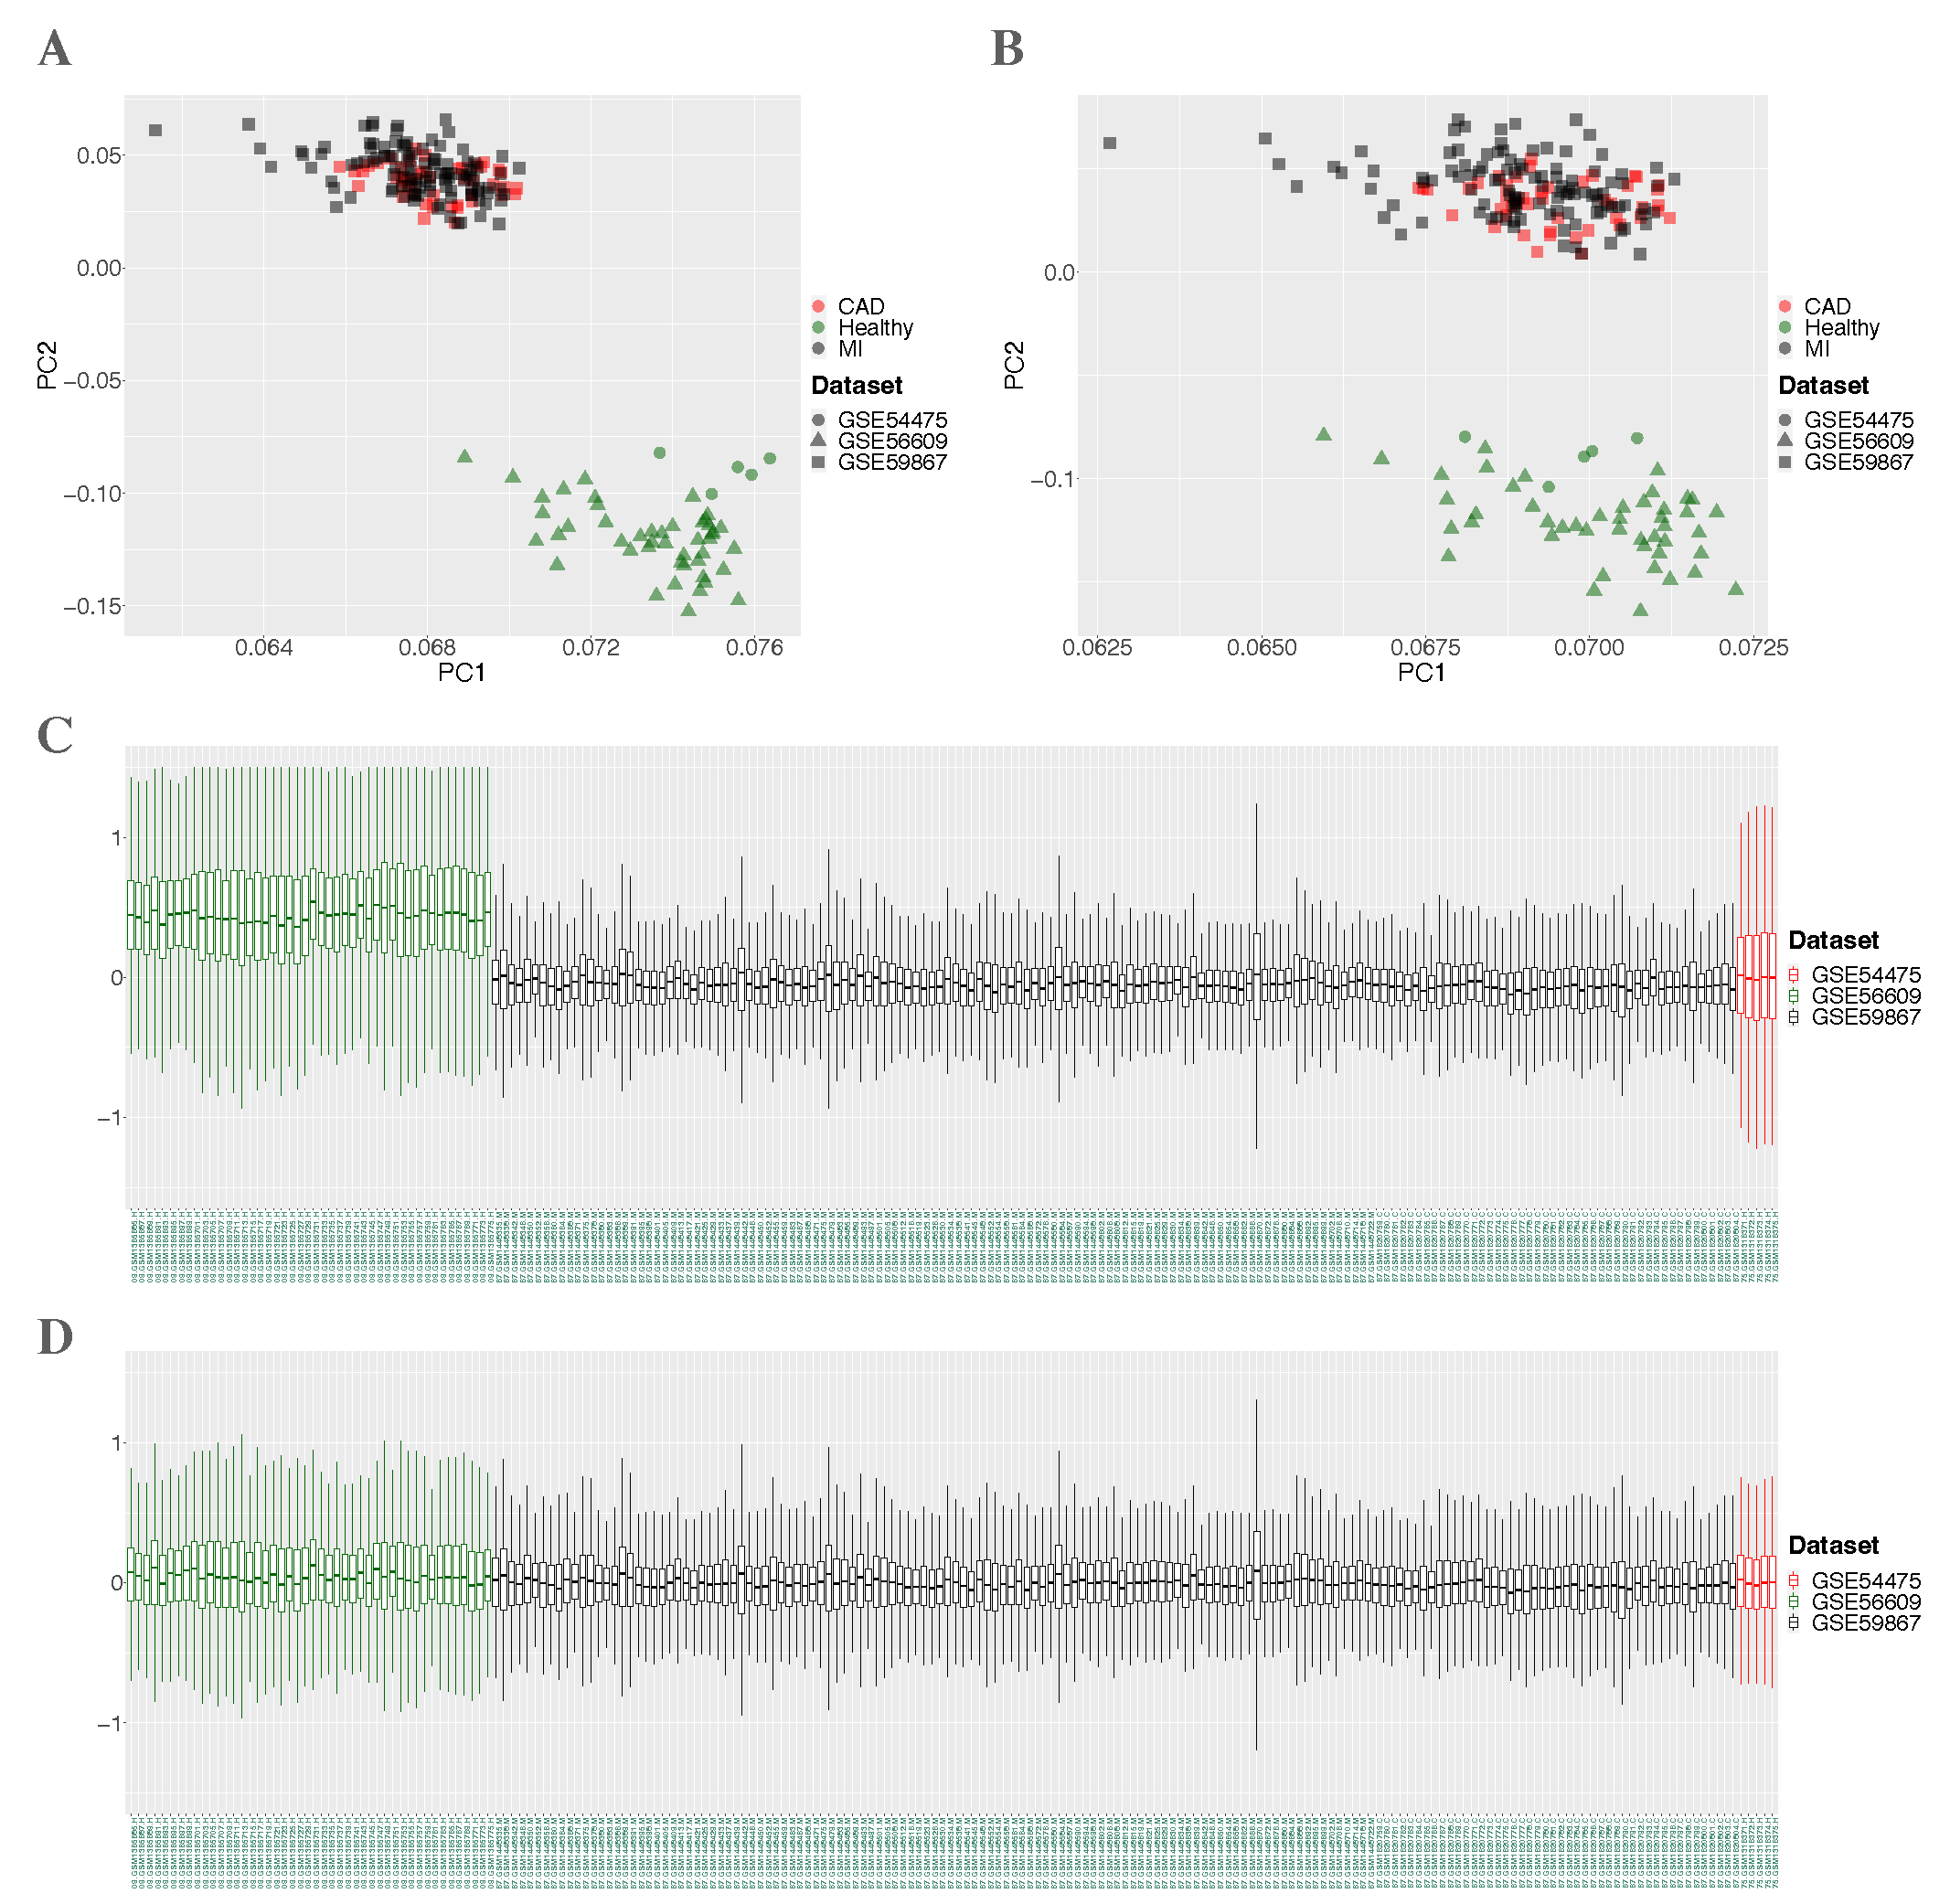
\includegraphics[width=1\linewidth]{../../DEG and DEM/Pics/PCA and RLE of trains} \caption{PCA and RLE plot for all samples before and after fRMA.}\label{fig:PCA}
\end{figure}

\hypertarget{differential-expression-analysis-1}{%
\subsection{Differential expression
analysis}\label{differential-expression-analysis-1}}

\begin{table}

\caption{\label{tab:DEGstab}Total, up-, and down-regulated DEGs and differentially expressed miRNAs.}
\centering
\begin{tabu} to \linewidth {>{\raggedright\arraybackslash}p{3cm}>{\centering}X>{\centering}X>{\centering}X>{\centering\arraybackslash}p{4cm}}
\toprule
  & DEGs & up-regulated DEGs & down-regulated DEGs & miRNAs\\
\midrule
MI vs. Healthy & 860 & 323 & 537 & hsa-miR-186, miR-21, miR-32\\
CAD vs. Healthy & 670 & 262 & 408 & hsa-miR-186, miR-21, miR-32\\
MI vs. CAD & 260 & 144 & 116 & hsa-miR-186\\
\bottomrule
\end{tabu}
\end{table}

According to the cutoff criterion of \(FDR < 0.05\), there were 860 DEGs
between the MI and the healthy samples. Among them, 323 were
up-regulated, and 537 were down-regulated in MI compared to the healthy
controls. In CAD and healthy groups comparison, we found 670 DEGs, of
which 262 and and 408 DEGs were up- and down-regulated, respectively in
CAD samples. In the MI and CAD groups, the number of DEGs was 260, and
the number of up- and down-regulated genes in MI samples were 144 and
116, respectively in comparison with CAD samples. These data are
summarized in Table @ref(tab:DEGstab).

\begin{figure}

{\centering \includegraphics[width=0.6\linewidth]{../../DEG and DEM/Pics/venny} 

}

\caption{Venn diagram for DEGs in CAD/Healthy, MI/Healthy, and MI/CAD comparison.}\label{fig:venn}
\end{figure}

The Venn diagram in Figure @ref(fig:venn) shows that CAD and MI samples
share a majority of their DEGs. From 860 DEGs of MI/healthy and 670 DEGs
of CAD/healthy, 531 genes were common which is 62\% of MI/healthy DEGs
and 79\% of CAD/healthy DEGs.

\hypertarget{gene-ontology-go-and-kyoto-encyclopedia-of-genes-and-genomes-kegg-enrichment-analyses-of-the-degs.}{%
\subsection{Gene ontology (GO) and Kyoto Encyclopedia of Genes and
Genomes (KEGG) enrichment analyses of the
DEGs.}\label{gene-ontology-go-and-kyoto-encyclopedia-of-genes-and-genomes-kegg-enrichment-analyses-of-the-degs.}}

To explore the biological classification of the DEGs, we performed GO
and KEGG pathway enrichment analyses on MI-healthy and CAD-healthy DEGs.
In MI versus healthy samples, GO enrichment analysis in the BP category,
suggested that the DEGs were enriched in ``immune response-regulating
signaling pathway'', ``lymphocyte differentiation'', ``immune
response-regulating cell surface receptor signaling pathway'', and
``leukocyte activation involved in immune response'' (Figure
@ref(fig:MIHEnrich)A). In the CC category, the DEGs were enriched in
``secretory granule membrane'', ``azurophil granule'', ``ficolin-1-rich
granule'', ``tertiary granule'', and ``ficolin-1-rich granule membrane''
(Figure @ref(fig:MIHEnrich)B). In the MF category, the DEGs were
involved in ``cadherin binding'' and ``MHC class I protein binding''
(Figure @ref(fig:MIHEnrich)C). KEGG pathway analysis indicated that the
DEGs were related to the following pathways: ``Chemokine signaling
pathway'', ``Lipid and atherosclerosis'', and ``Hematopoietic cell
lineage'' (Figure @ref(fig:MIHEnrich)D).

\begin{figure}
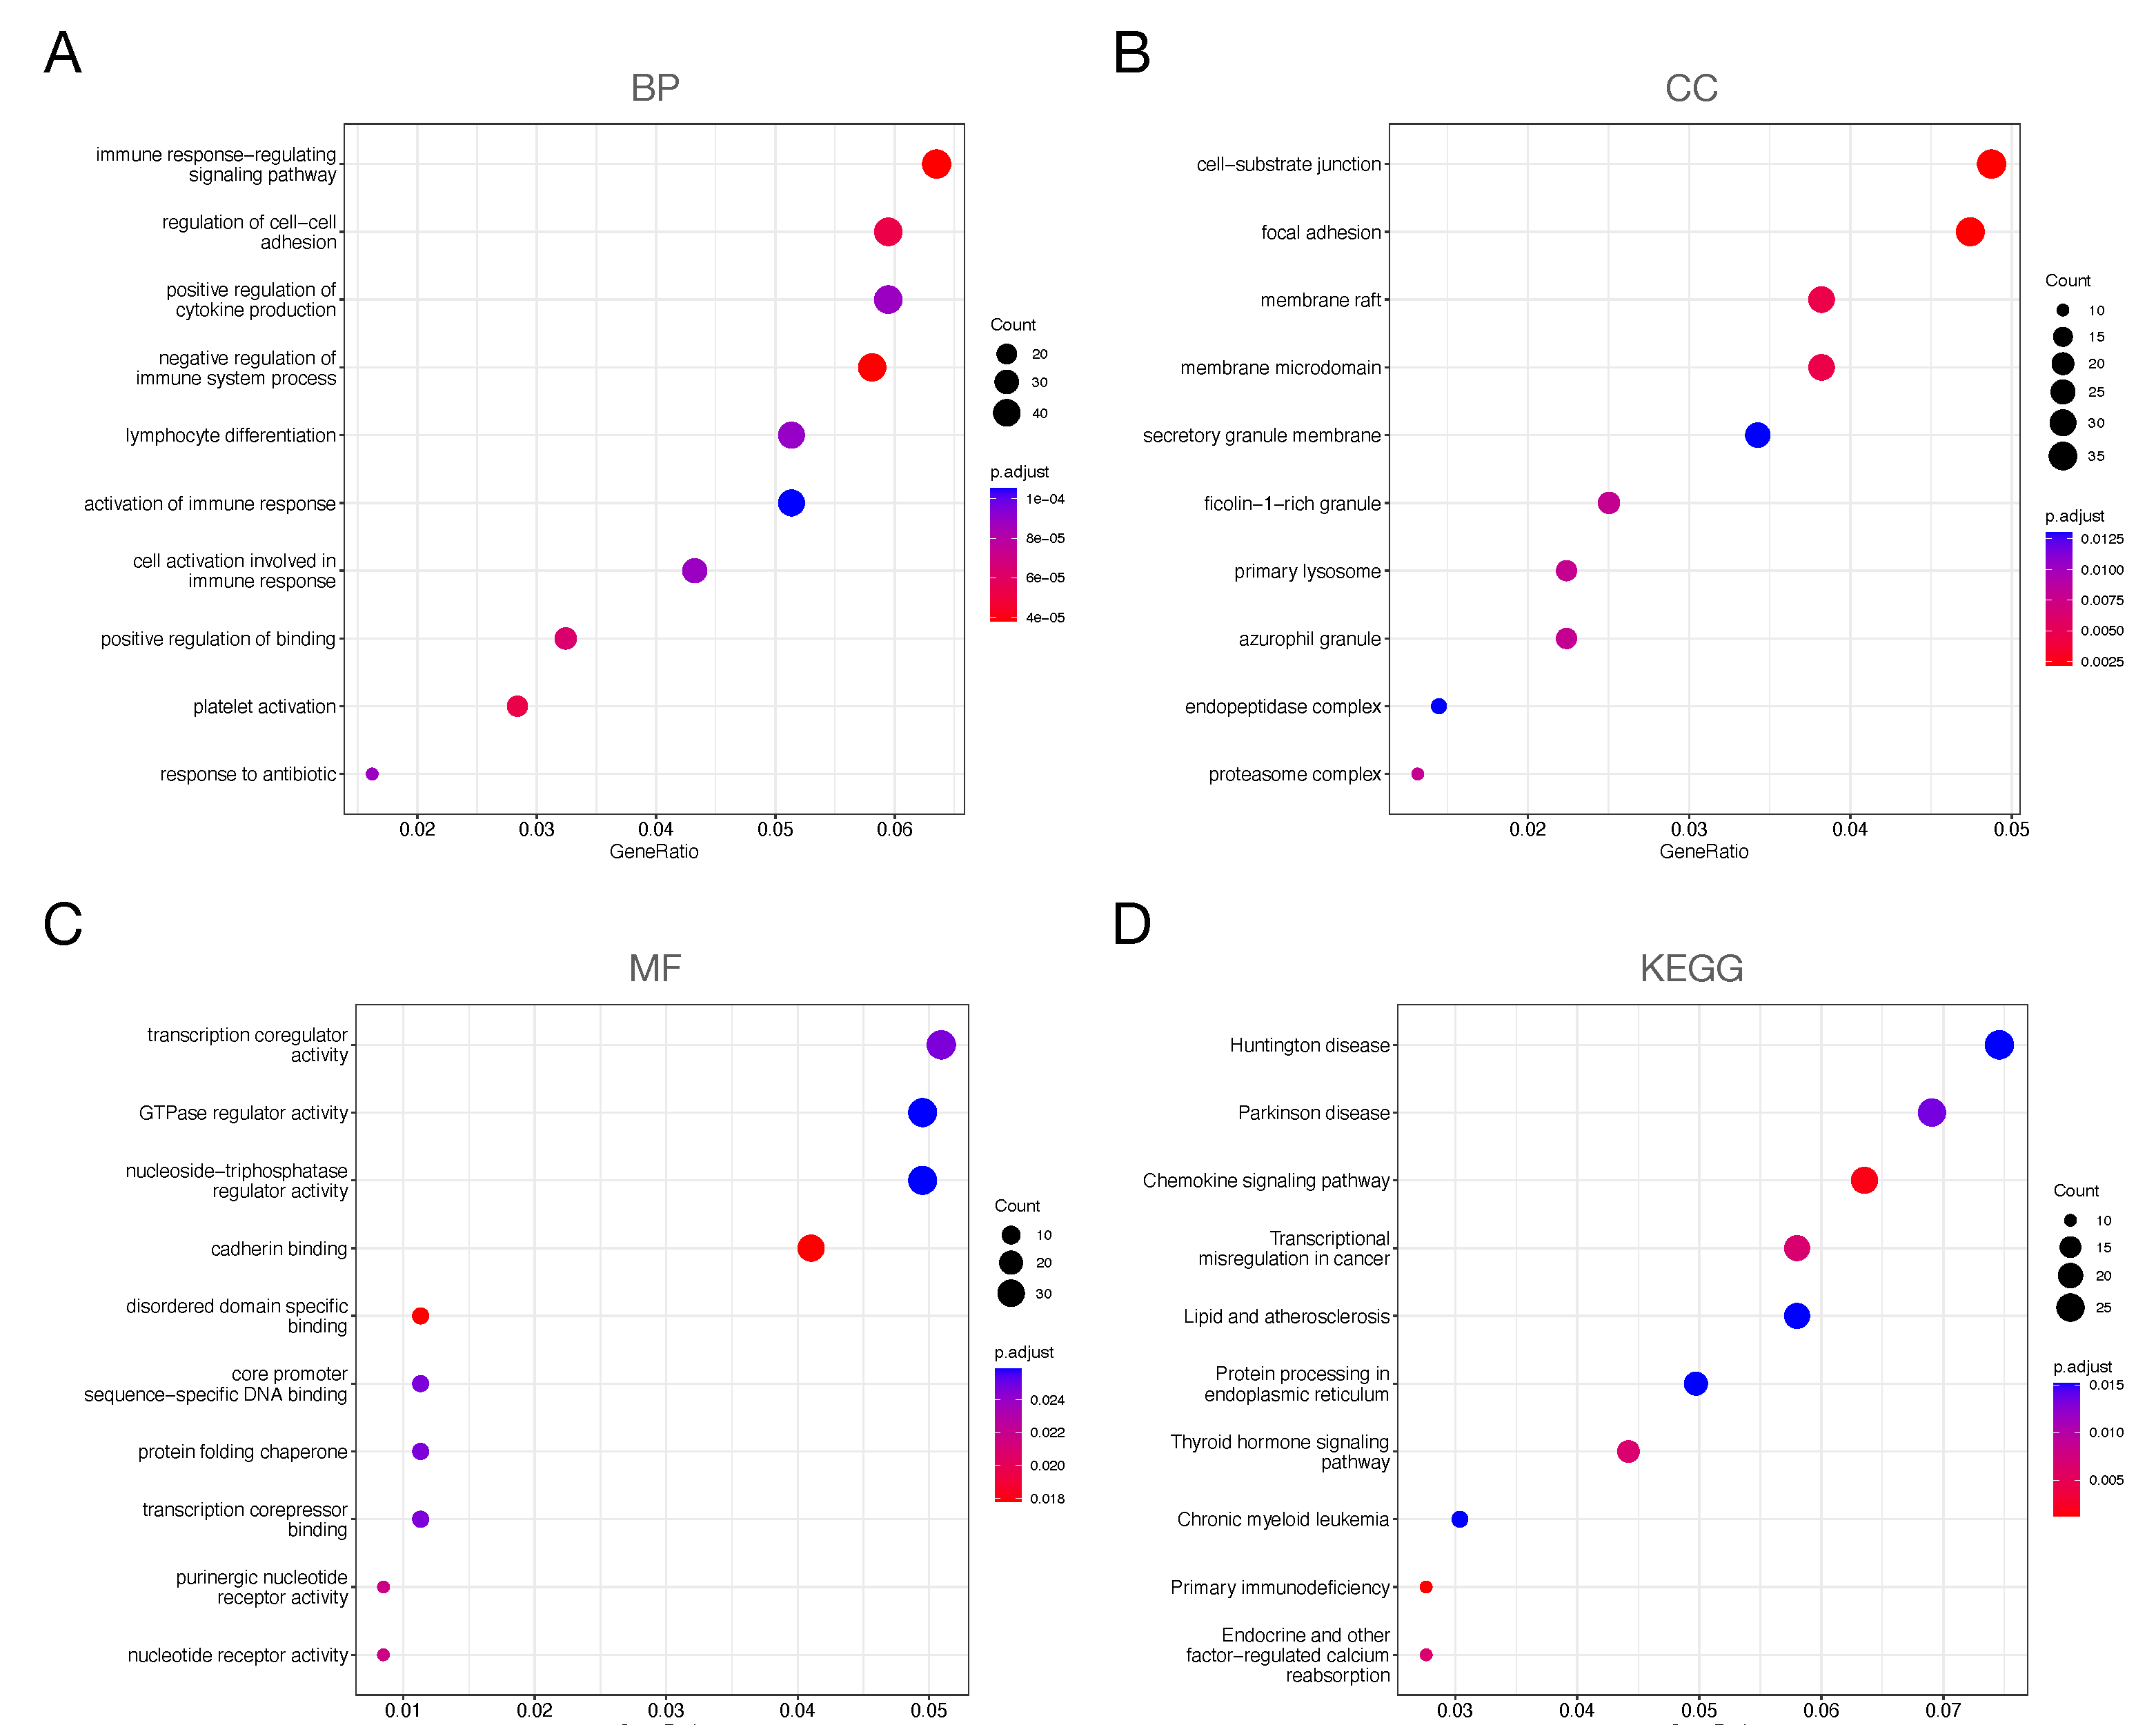
\includegraphics[width=0.95\linewidth]{../../DEG and DEM/Pics/enrich MI-Healthy} \caption{Gene Ontology (GO) and Kyoto Encyclopedia of Genes and Genomes (KEGG) pathways enriched with the MI and healthy DEGs. (A) Biological process terms. (B) Cellular component terms. (C) Molecular function terms. (D) KEGG analysis.}\label{fig:MIHEnrich}
\end{figure}

The enrichment results for DEGs of CAD versus healthy samples were as
follows. In the BP category, GO enrichment suggested that the DEGs were
enriched in ``positive regulation of defense response'', ``positive
regulation of innate immune response'', ``mononuclear cell
differentiation'', and ``positive regulation of response to external
stimulus'' (Figure @ref(fig:CADHEnrich)A). In the CC category, the DEGs
were enriched in ``azurophil granule'', ``ficolin-1-rich granule'', and
``ficolin-1-rich granule membrane'' (Figure @ref(fig:CADHEnrich)B). In
the MF category, the DEGs were involved in ``lipoprotein particle
receptor binding'' and ``NF-\(\kappa\)B binding'' (Figure
@ref(fig:CADHEnrich)C). KEGG pathway analysis indicated that the DEGs
were related to the following pathways: ``Chemokine signaling pathway'',
``Lipid and atherosclerosis'', and ``Hematopoietic cell lineage''
(Figure @ref(fig:CADHEnrich)D).

\begin{figure}
\includegraphics[width=0.95\linewidth]{../../DEG and DEM/Pics/enrich CAD-Healthy} \caption{Gene Ontology (GO) and Kyoto Encyclopedia of Genes and Genomes (KEGG) pathways enriched with the CAD and healthy DEGs. (A) Biological process terms. (B) Cellular component terms. (C) Molecular function terms. (D) KEGG analysis.}\label{fig:CADHEnrich}
\end{figure}

\hypertarget{machine-learning}{%
\subsection{Machine Learning}\label{machine-learning}}

\hypertarget{mirnas-in-degs-1}{%
\subsubsection{miRNAs in DEGs}\label{mirnas-in-degs-1}}

Among all DEGs, just miR-186, miR-32, and miR-21 were detected as
differentially expressed miRNAs. The expression profile of these three
miRNAs is presented in Figure @ref(fig:DEMexp). Additionally, The ROC
curves of each miRNA for each layer are presented in Figure
@ref(fig:miRROC). Using the logistic regression model the AUC for
miR-21, miR-32, and miR-186 was 0.99, 1, and 0.91 respectively (Figure
@ref(fig:miRROC)A). Besides, the accuracy of each miRNA for classifying
the samples into healthy and not-healthy groups on the test set was
0.92, 0.98, and 0.89 for miR-21, miR-32, and miR-186, respectively.
Moreover, the ROC curve of each miRNA for classifying MI and CAD samples
was presented in Figure @ref(fig:miRROC)B. For miR-21, miR-32, and
miR-186, the AUC and accuracy on the test set were 0.85; 0.7; and 0.82,
and 0.78; 0.67; and 0.74, respectively.

\begin{table}

\caption{\label{tab:mirExptable}Target miRNAs log fold-change and adjusted p-values for CAD samples relative to healthy, MI samples relative to healthy, and MI samples relative to CAD.}
\centering
\begin{tabu} to \linewidth {>{\raggedright}X>{\centering}X>{\centering}X>{\centering}X>{\centering}X>{\centering}X>{\centering}X}
\toprule
\multicolumn{1}{c}{ } & \multicolumn{2}{c}{CAD/Healthy} & \multicolumn{2}{c}{MI/Healthy} & \multicolumn{2}{c}{MI/CAD} \\
\cmidrule(l{3pt}r{3pt}){2-3} \cmidrule(l{3pt}r{3pt}){4-5} \cmidrule(l{3pt}r{3pt}){6-7}
  & logFC & adj. p-value & logFC & adj. p-value & logFC & adj. p-value\\
\midrule
miR-186 & 1.4 & 3.60e-25 & 0.9 & 6.76e-20 & -0.5 & 1.05e-09\\
miR-21 & 1.4 & 1.31e-17 & 2.3 & 2.07e-47 & 0.8 & 2.96e-11\\
miR-32 & 2.5 & 8.39e-43 & 2.2 & 3.10e-59 & -0.3 & 7.60e-04\\
miR-155 & -0.6 & 2.49e-12 & -0.9 & 7.59e-33 & -0.2 & 2.68e-07\\
miR-142 & 0.2 & 1.90e-01 & -0.1 & 1.70e-01 & -0.3 & 2.90e-04\\
miR-197 & 0.5 & 2.95e-20 & 0.7 & 1.59e-47 & 0.2 & 8.58e-09\\
miR-29A & 0.7 & 7.76e-29 & 0.1 & 1.70e-01 & -0.5 & 2.14e-10\\
miR-320C1 & 0.8 & 4.72e-22 & 0.5 & 1.89e-30 & -0.2 & 1.84e-05\\
\bottomrule
\end{tabu}
\end{table}

\begin{figure}

{\centering \includegraphics[width=0.5\linewidth]{../../ML/Pics/DEGs healthy not-healthy/DEMs Expression} 

}

\caption{Expression profile of miR-186, miR-21, and miR32 in Healthy, CAD, and MI samples.}\label{fig:DEMexp}
\end{figure}

\begin{figure}

{\centering 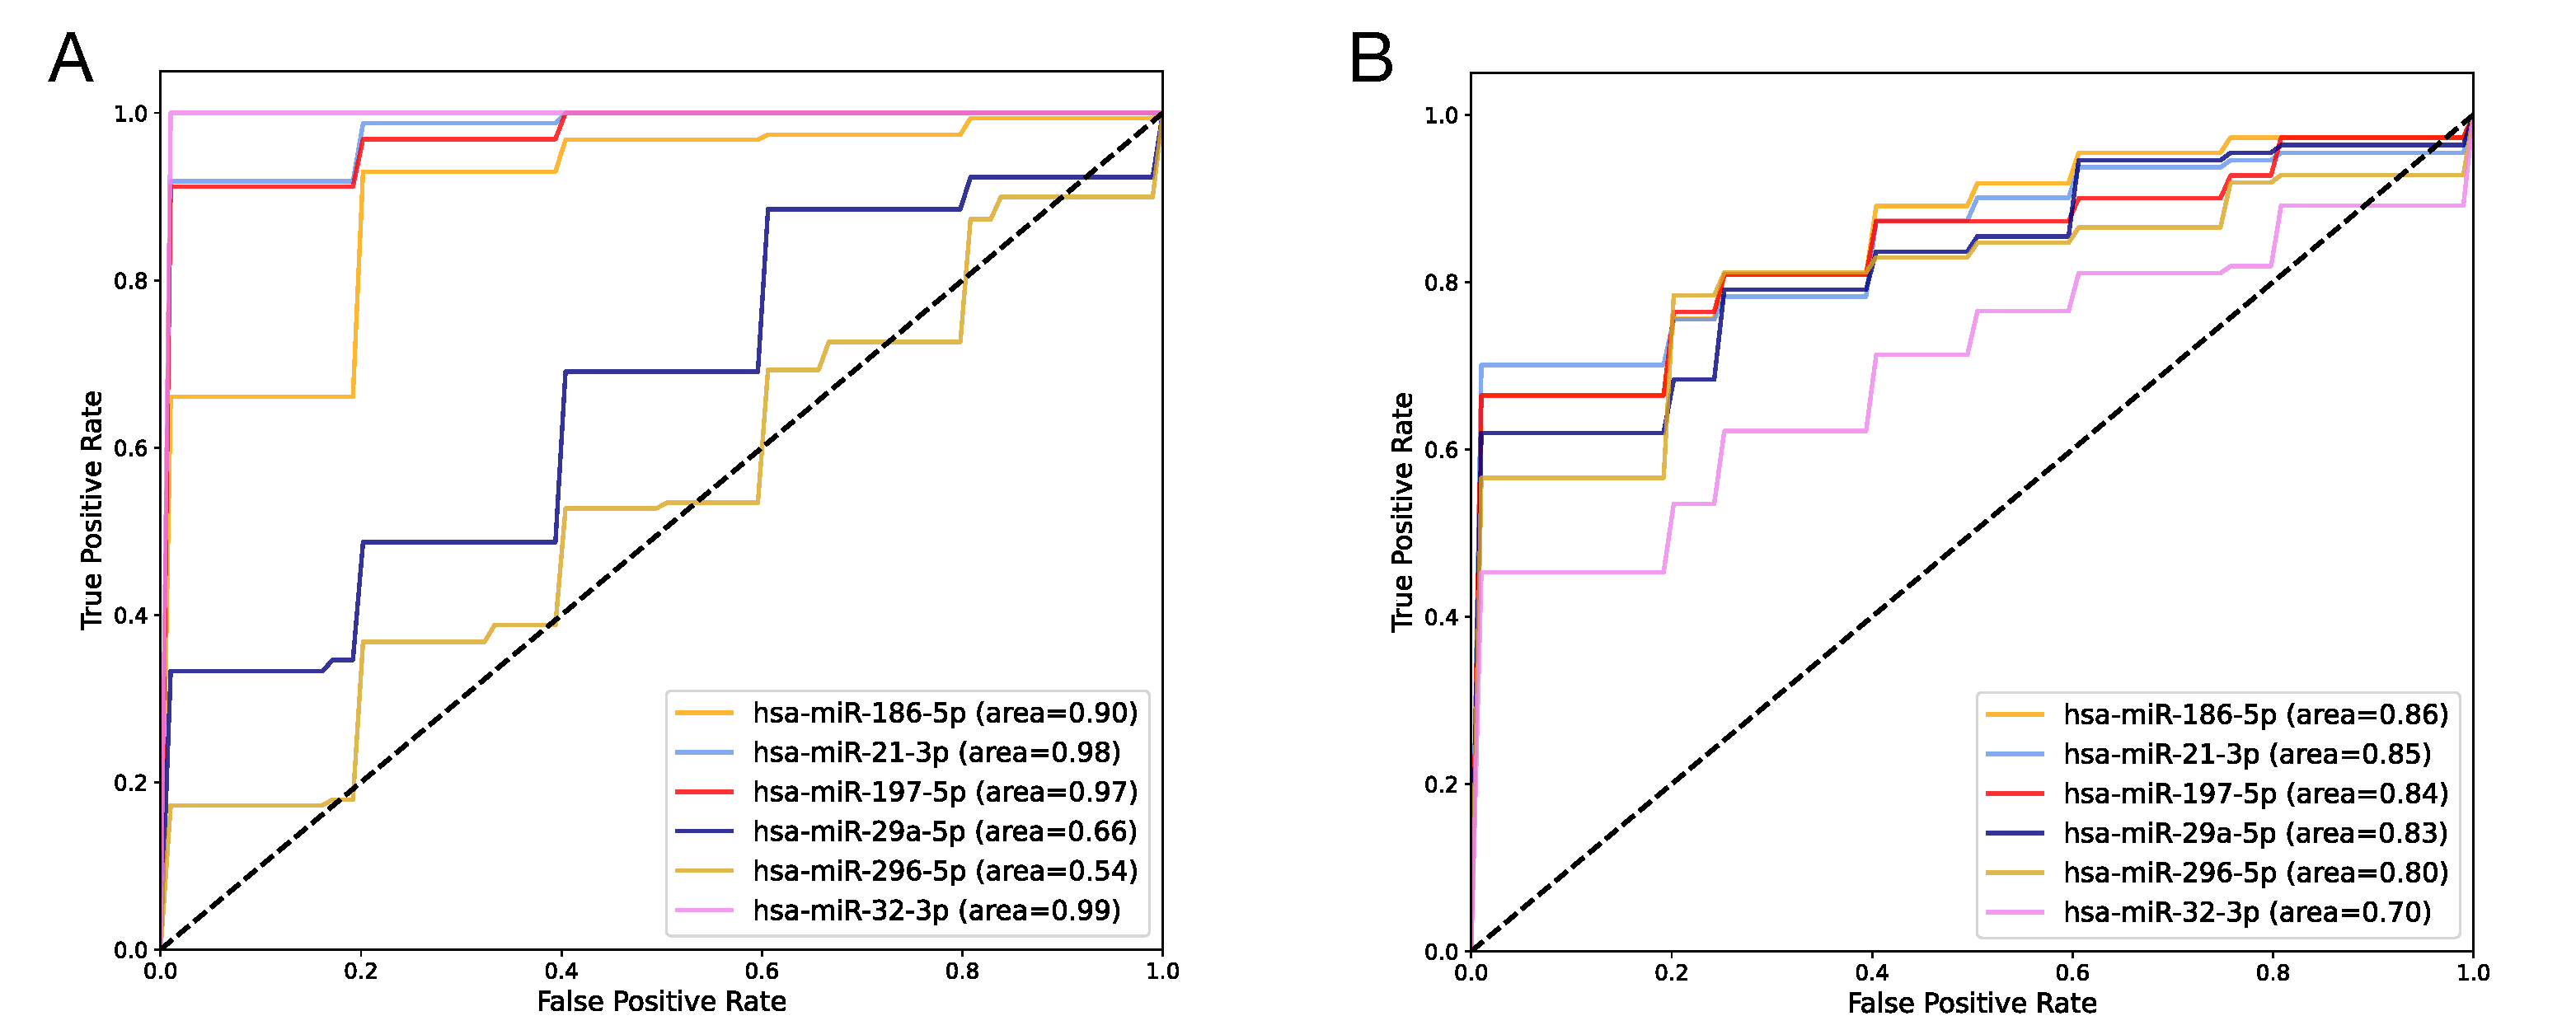
\includegraphics[width=0.95\linewidth]{../../ML/Pics/miRs ROCs} 

}

\caption{ROC curve for single miRNAs on test set classification for (A) healthy and not-healthy samples and (B) CAD and MI samples.}\label{fig:miRROC}
\end{figure}

\hypertarget{first-layer-for-healthy-not-healthy-isolation}{%
\paragraph{First layer for healthy not-healthy
isolation:}\label{first-layer-for-healthy-not-healthy-isolation}}

Although single miRNAs had acceptable performance, their predictive
value could be improved even further by using them as a set. The ROC
curve for the SVM model with an RBF kernel trained with all three miRNAs
is presented in Figure @ref(fig:DEMROC)A. The model had a better
performance in classification than single miRNAs.The AUC for the model
is 1, and its accuracy on the test set was also 1. In Figure
@ref(fig:DEMCF)A, the confusion matrix for the model is presented.

\begin{figure}

{\centering 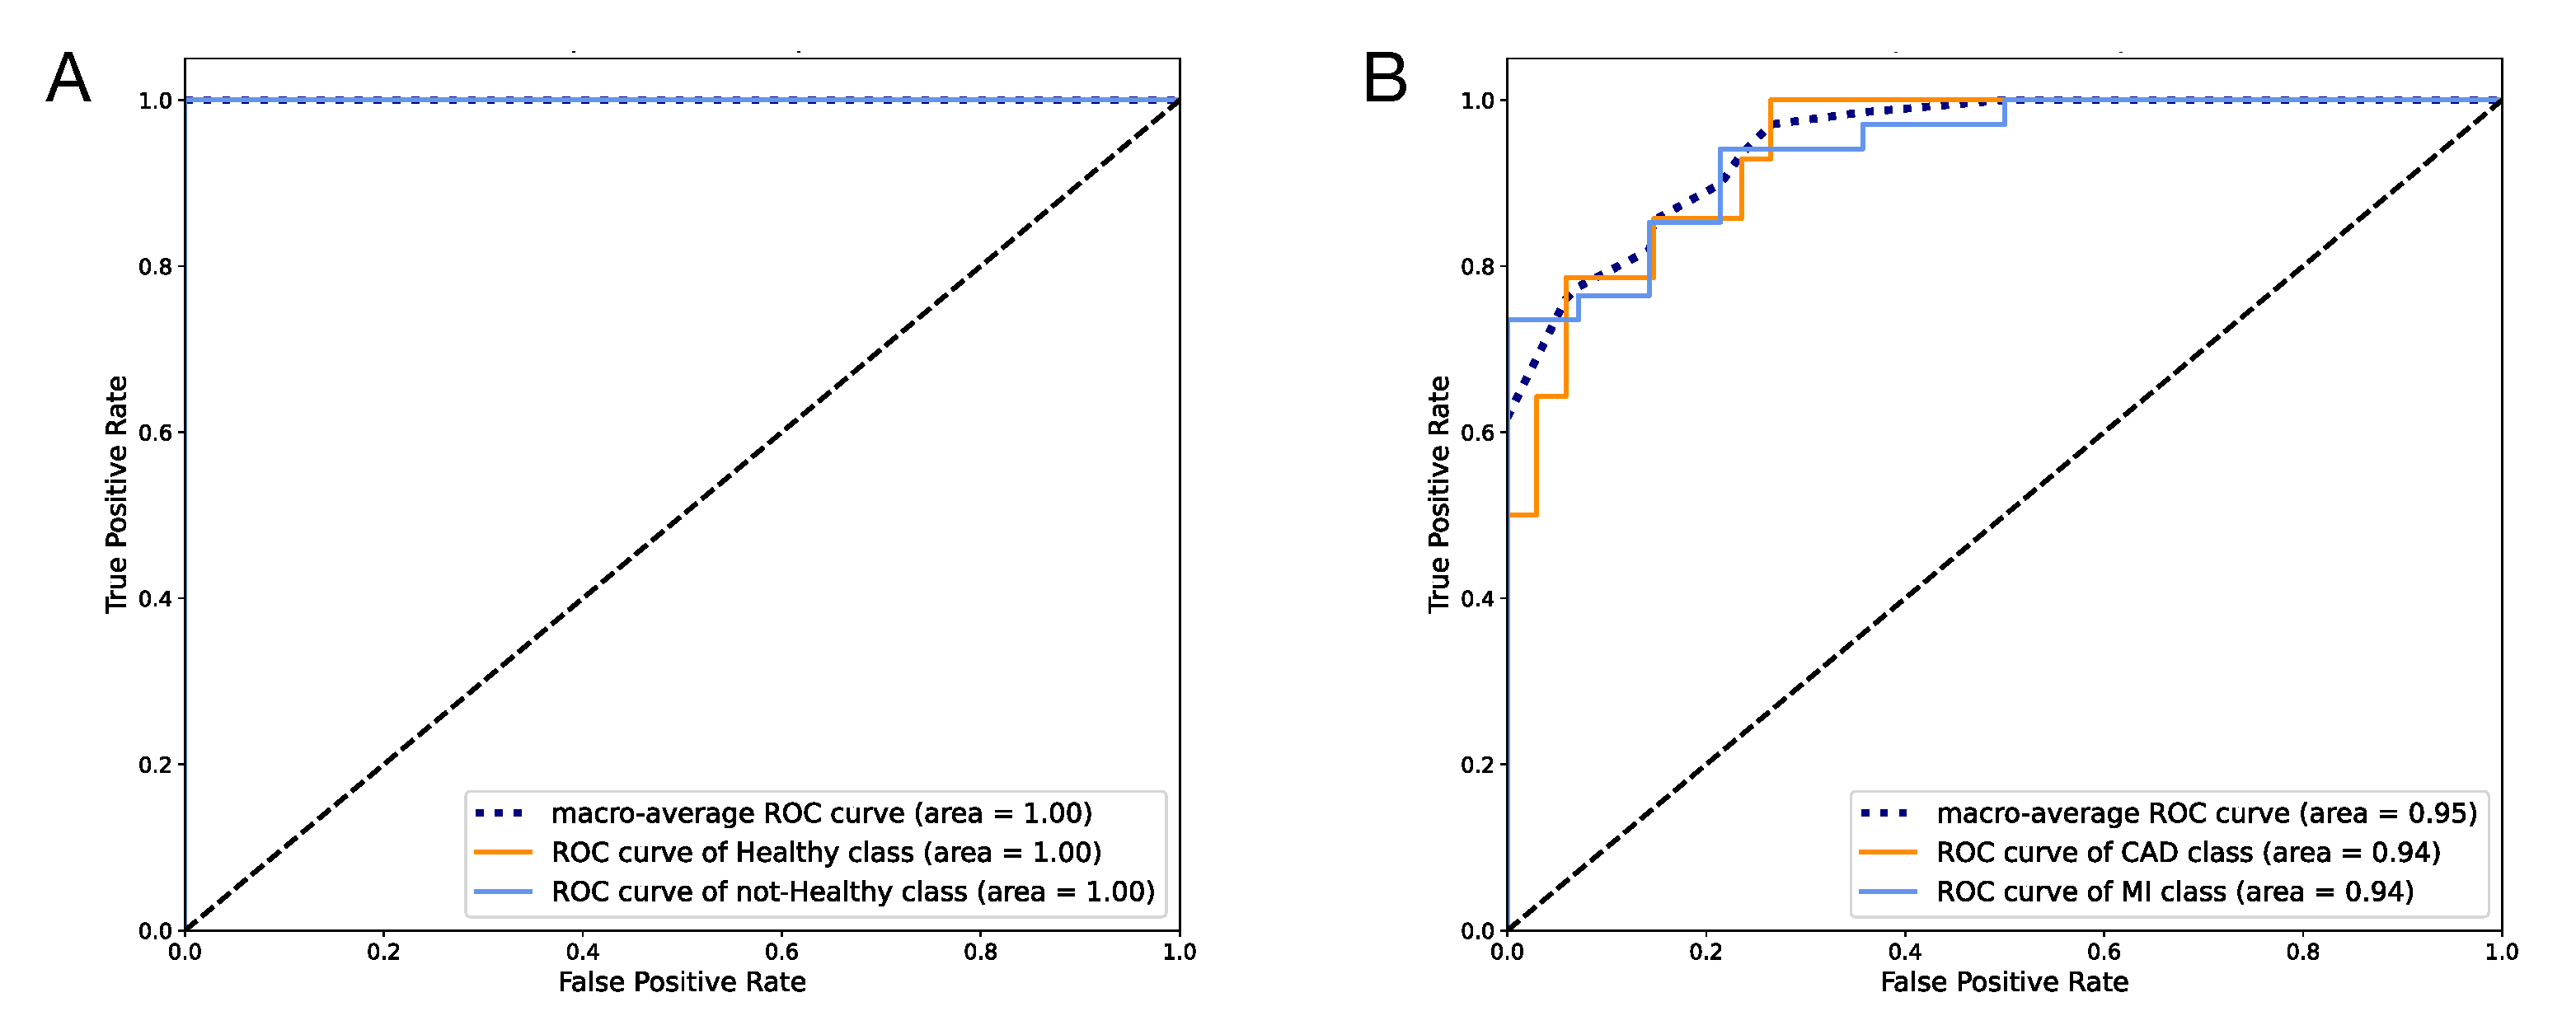
\includegraphics[width=0.95\linewidth]{../../ML/Pics/DEMs ROCs h not h cad mi} 

}

\caption{ROC curve for miRNAs in DEGs on test set classification for (A) healthy and not-healthy samples and (B) CAD and MI samples.}\label{fig:DEMROC}
\end{figure}

\begin{figure}

{\centering 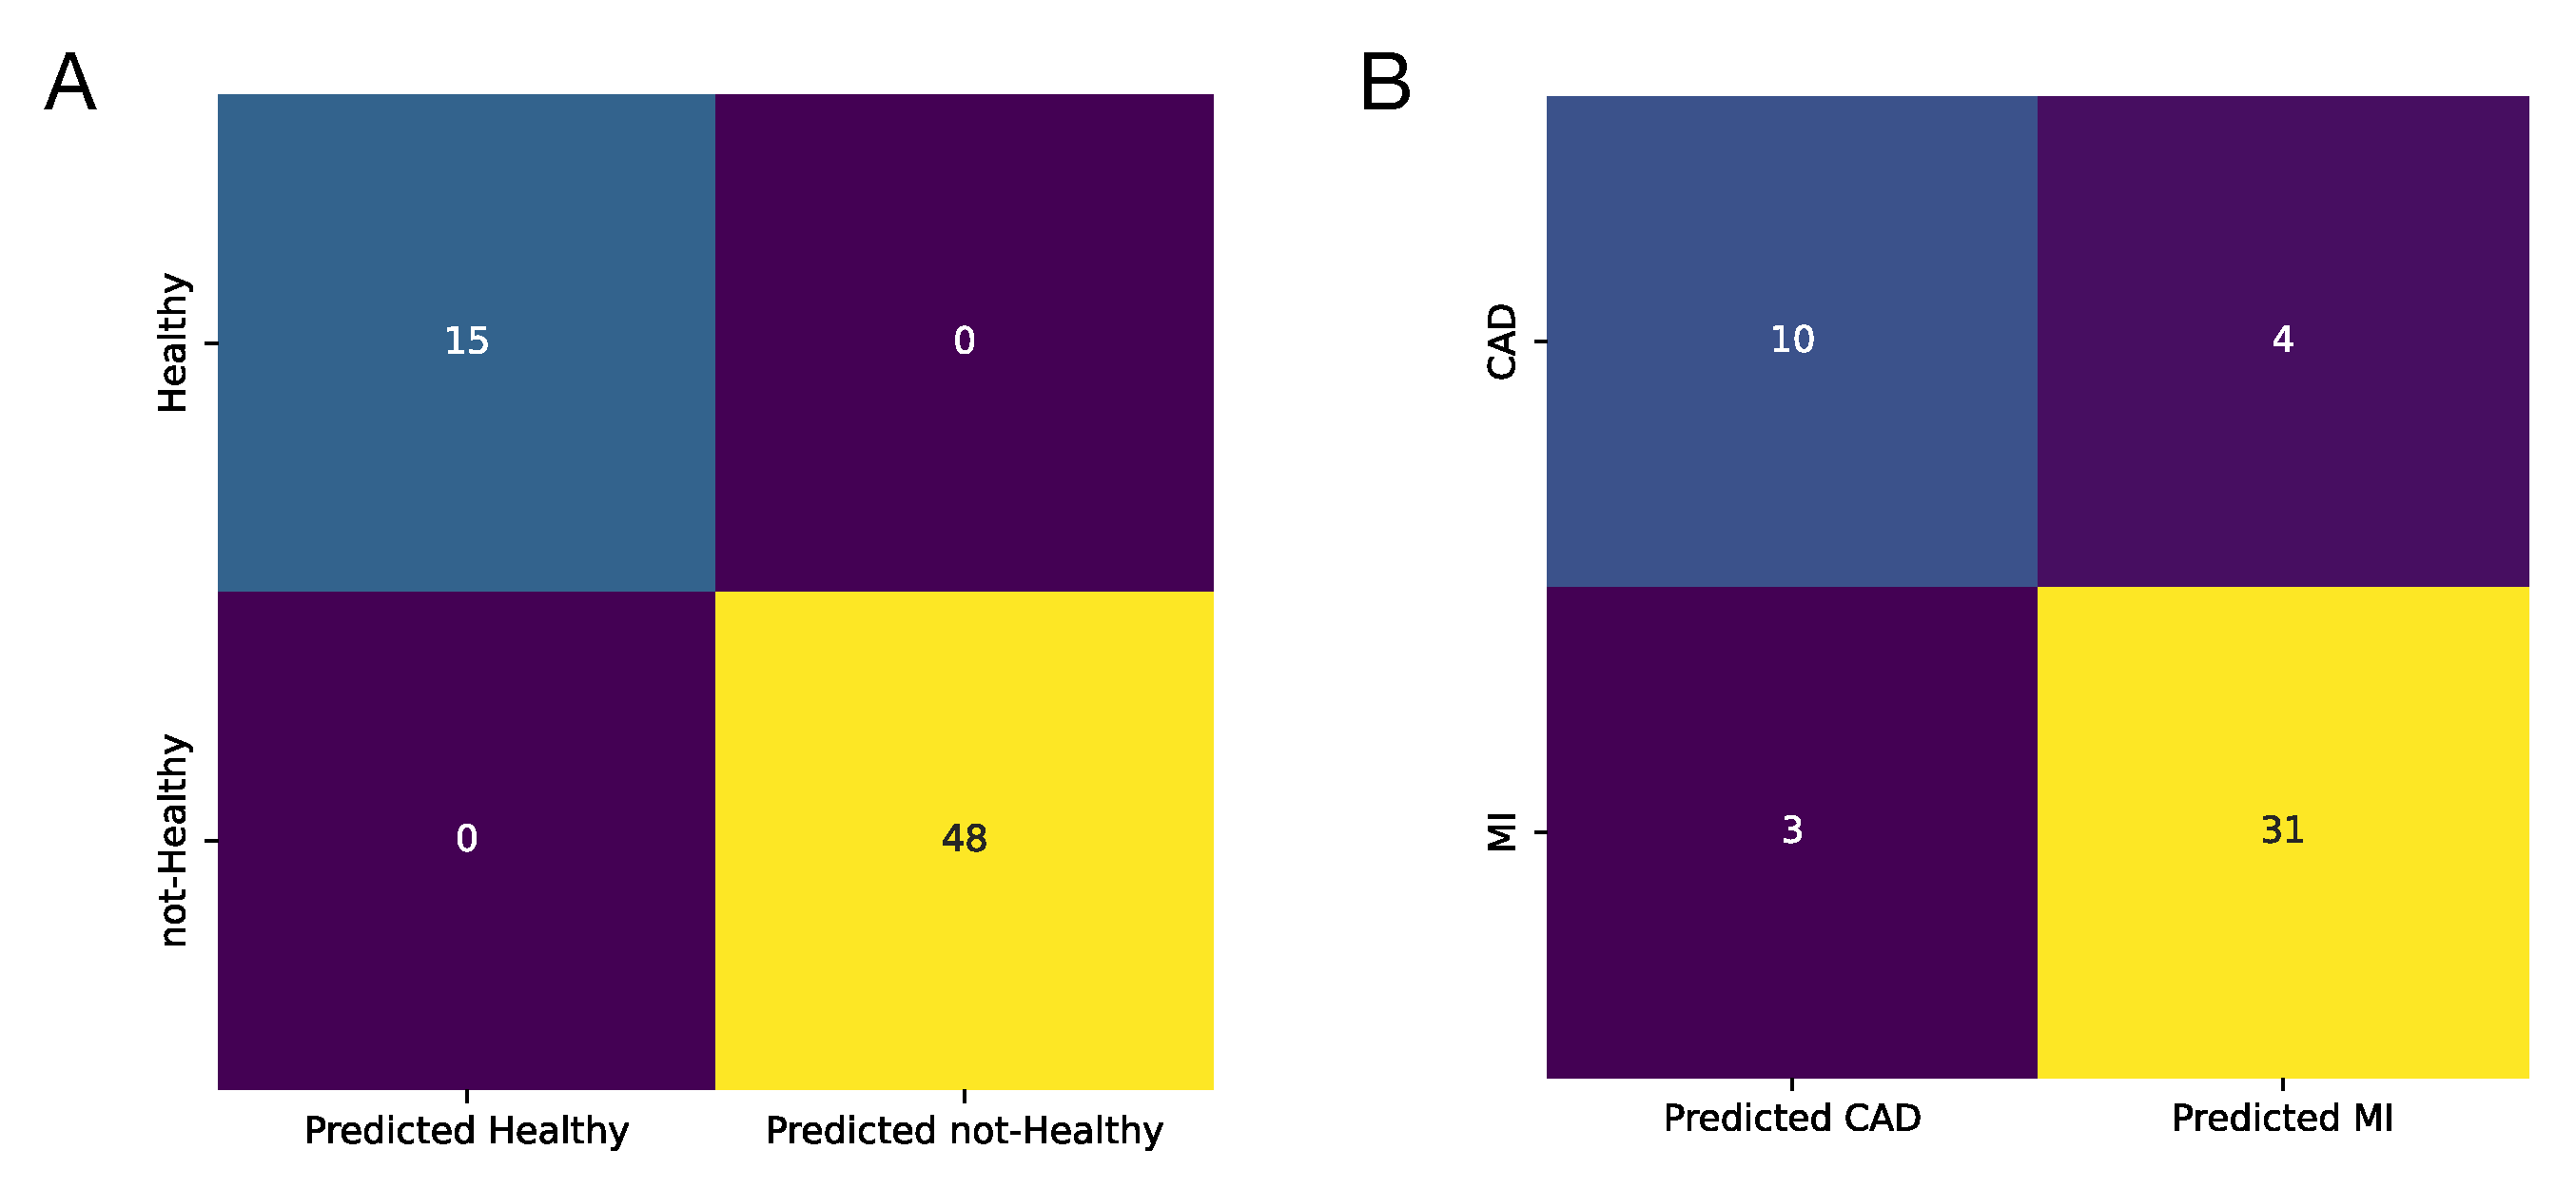
\includegraphics[width=0.9\linewidth]{../../ML/Pics/DEMs Conf. matrix} 

}

\caption{Confusion matrix on the test set for (A) An SVM model with RBF kernel for healthy and not-healthy and (B) An SVM model with linear kernel for CAD and MI samples classification.}\label{fig:DEMCF}
\end{figure}

\hypertarget{second-layer-for-separating-mi-samples-from-cad}{%
\paragraph{Second layer for separating MI samples from
CAD:}\label{second-layer-for-separating-mi-samples-from-cad}}

Different models were trained using expression values for three
differentially miRNAs. The models' 10-fold cross-validated AUC and
accuracy on the test set are reported in Figure @ref(fig:DEMmodels). The
best model from both AUC and accuracy point-of-view was the SVM model
with linear kernel. The AUC and accuracy for this model with its pre-set
values were 0.93 and 0.82 respectively. The model was hyper-tuned for C
and gamma hyper-parameters, and therefore the model showed better
performance. The ROC curve of the hyper-tuned model is presented in
Figure @ref(fig:DEMROC)B. For this model the AUC reached 0.95 and the
accuracy improved to 0.85 (Table @ref(tab:DEGsML)). Moreover, the
sensitivity and specificity for the model on the test set were 0.91 and
0.71 respectively. The confusion matrix for the hyper-tuned model is
illustrated in Figure @ref(fig:DEMCF)B.

\begin{figure}

{\centering 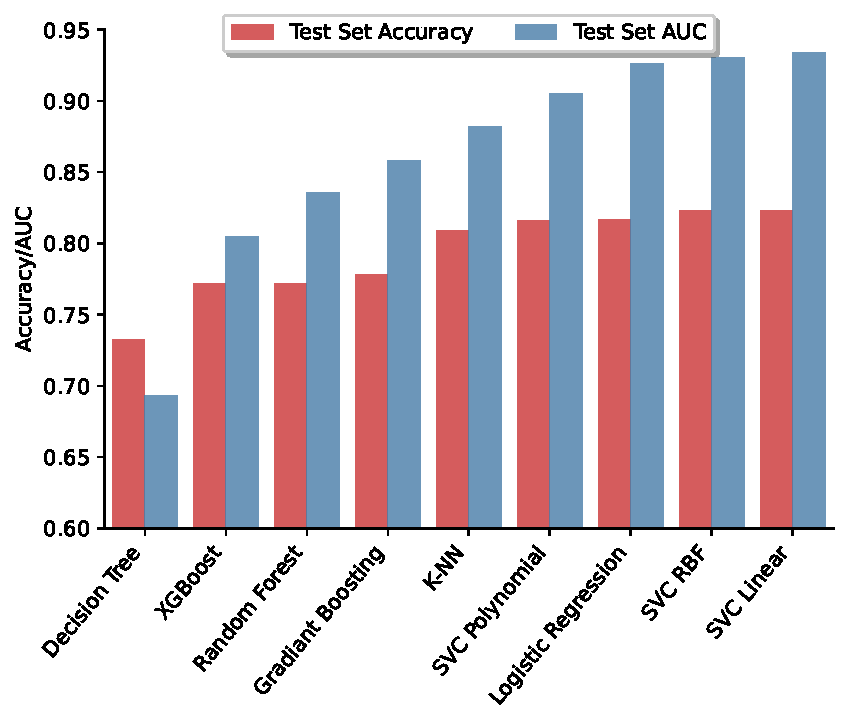
\includegraphics[width=0.65\linewidth]{../../ML/Pics/Models DEGs mirs} 

}

\caption{Area under the curve (AUC) and accuracy of different models trained with three miRNAs in DEGs on the test set.}\label{fig:DEMmodels}
\end{figure}

\begin{table}

\caption{\label{tab:DEGsML}AUC-ROC and accuracy for SVM with the linear kernel as the best model trained with differentially expressed miRNAs on the train and test set before and after hyper-tuning}
\centering
\begin{tabu} to \linewidth {>{\centering}X>{\centering}X>{\centering}X>{\centering}X>{\centering}X>{\centering}X}
\toprule
\multicolumn{2}{c}{ } & \multicolumn{2}{c}{Pre-set parameters} & \multicolumn{2}{c}{Hyper-tuned} \\
\cmidrule(l{3pt}r{3pt}){3-4} \cmidrule(l{3pt}r{3pt}){5-6}
Model & Metrics & train & test & train & test\\
\midrule
SVM & AUC-ROC & 0.91 & 0.93 & 0.92 & 0.95\\
(Linear Kernel) & Accuracy & 0.83 & 0.82 & 0.84 & 0.85\\
\bottomrule
\end{tabu}
\end{table}

\hypertarget{auc-approach}{%
\subsubsection{AUC approach}\label{auc-approach}}

After calculating the AUC for each miRNA for the classification of MI
and CAD samples, miRNAs were sorted, and their performance was
investigated as a set. The metric of choice for selecting the best set
was AUC. As shown in Figure @ref(fig:AUCset), the AUC increased until
the number of miRNAs in the set reached six, and after that, it dropped.
The AUC for separating MI samples from CAD using these miRNAs was 0.93.
The miRNAs in the set were miR-29a, miR-197, miR-142, miR-21, miR-155,
and miR-320C1. The expression values of these miRNAs in healthy, CAD,
and MI samples are presented in Figure @ref(fig:AUCexp). The ROC curve
of the selected miRNAs for MI and CAD sample classification is
illustrated in Figure @ref(fig:miRROC)B.

\begin{figure}

{\centering \includegraphics[width=0.65\linewidth]{../../ML/Pics/AUC for cad mi mirs} 

}

\caption{Area under the curve (AUC) for sets containing an increasing number of miRNAs with the highest individual AUC in MI/CAD separation.}\label{fig:AUCset}
\end{figure}

\begin{figure}

{\centering \includegraphics[width=0.9\linewidth]{../../ML/Pics/ExpressionforAUC} 

}

\caption{Expression profile of has-miR-29A, has-miR-197, has-miR-142, has-miR-21, has-miR-155, and has-miR-320C1 in Healthy, CAD, and MI samples.}\label{fig:AUCexp}
\end{figure}

\hypertarget{first-layer-for-isolation-of-healthy-and-not-healthy-samples-1}{%
\paragraph{First layer for isolation of healthy and not-healthy
samples}\label{first-layer-for-isolation-of-healthy-and-not-healthy-samples-1}}

Using the selected set, an SVM model with an RBF kernel was trained to
separate healthy from not-healthy samples. The ROC curve for the model
is presented in Figure @ref(fig:AUCROC)A and the confusion matrix is
illustrated in Figure @ref(fig:AUCCF)A. Both AUC and accuracy for the
model on the test set were equal to 1.

\begin{figure}

{\centering 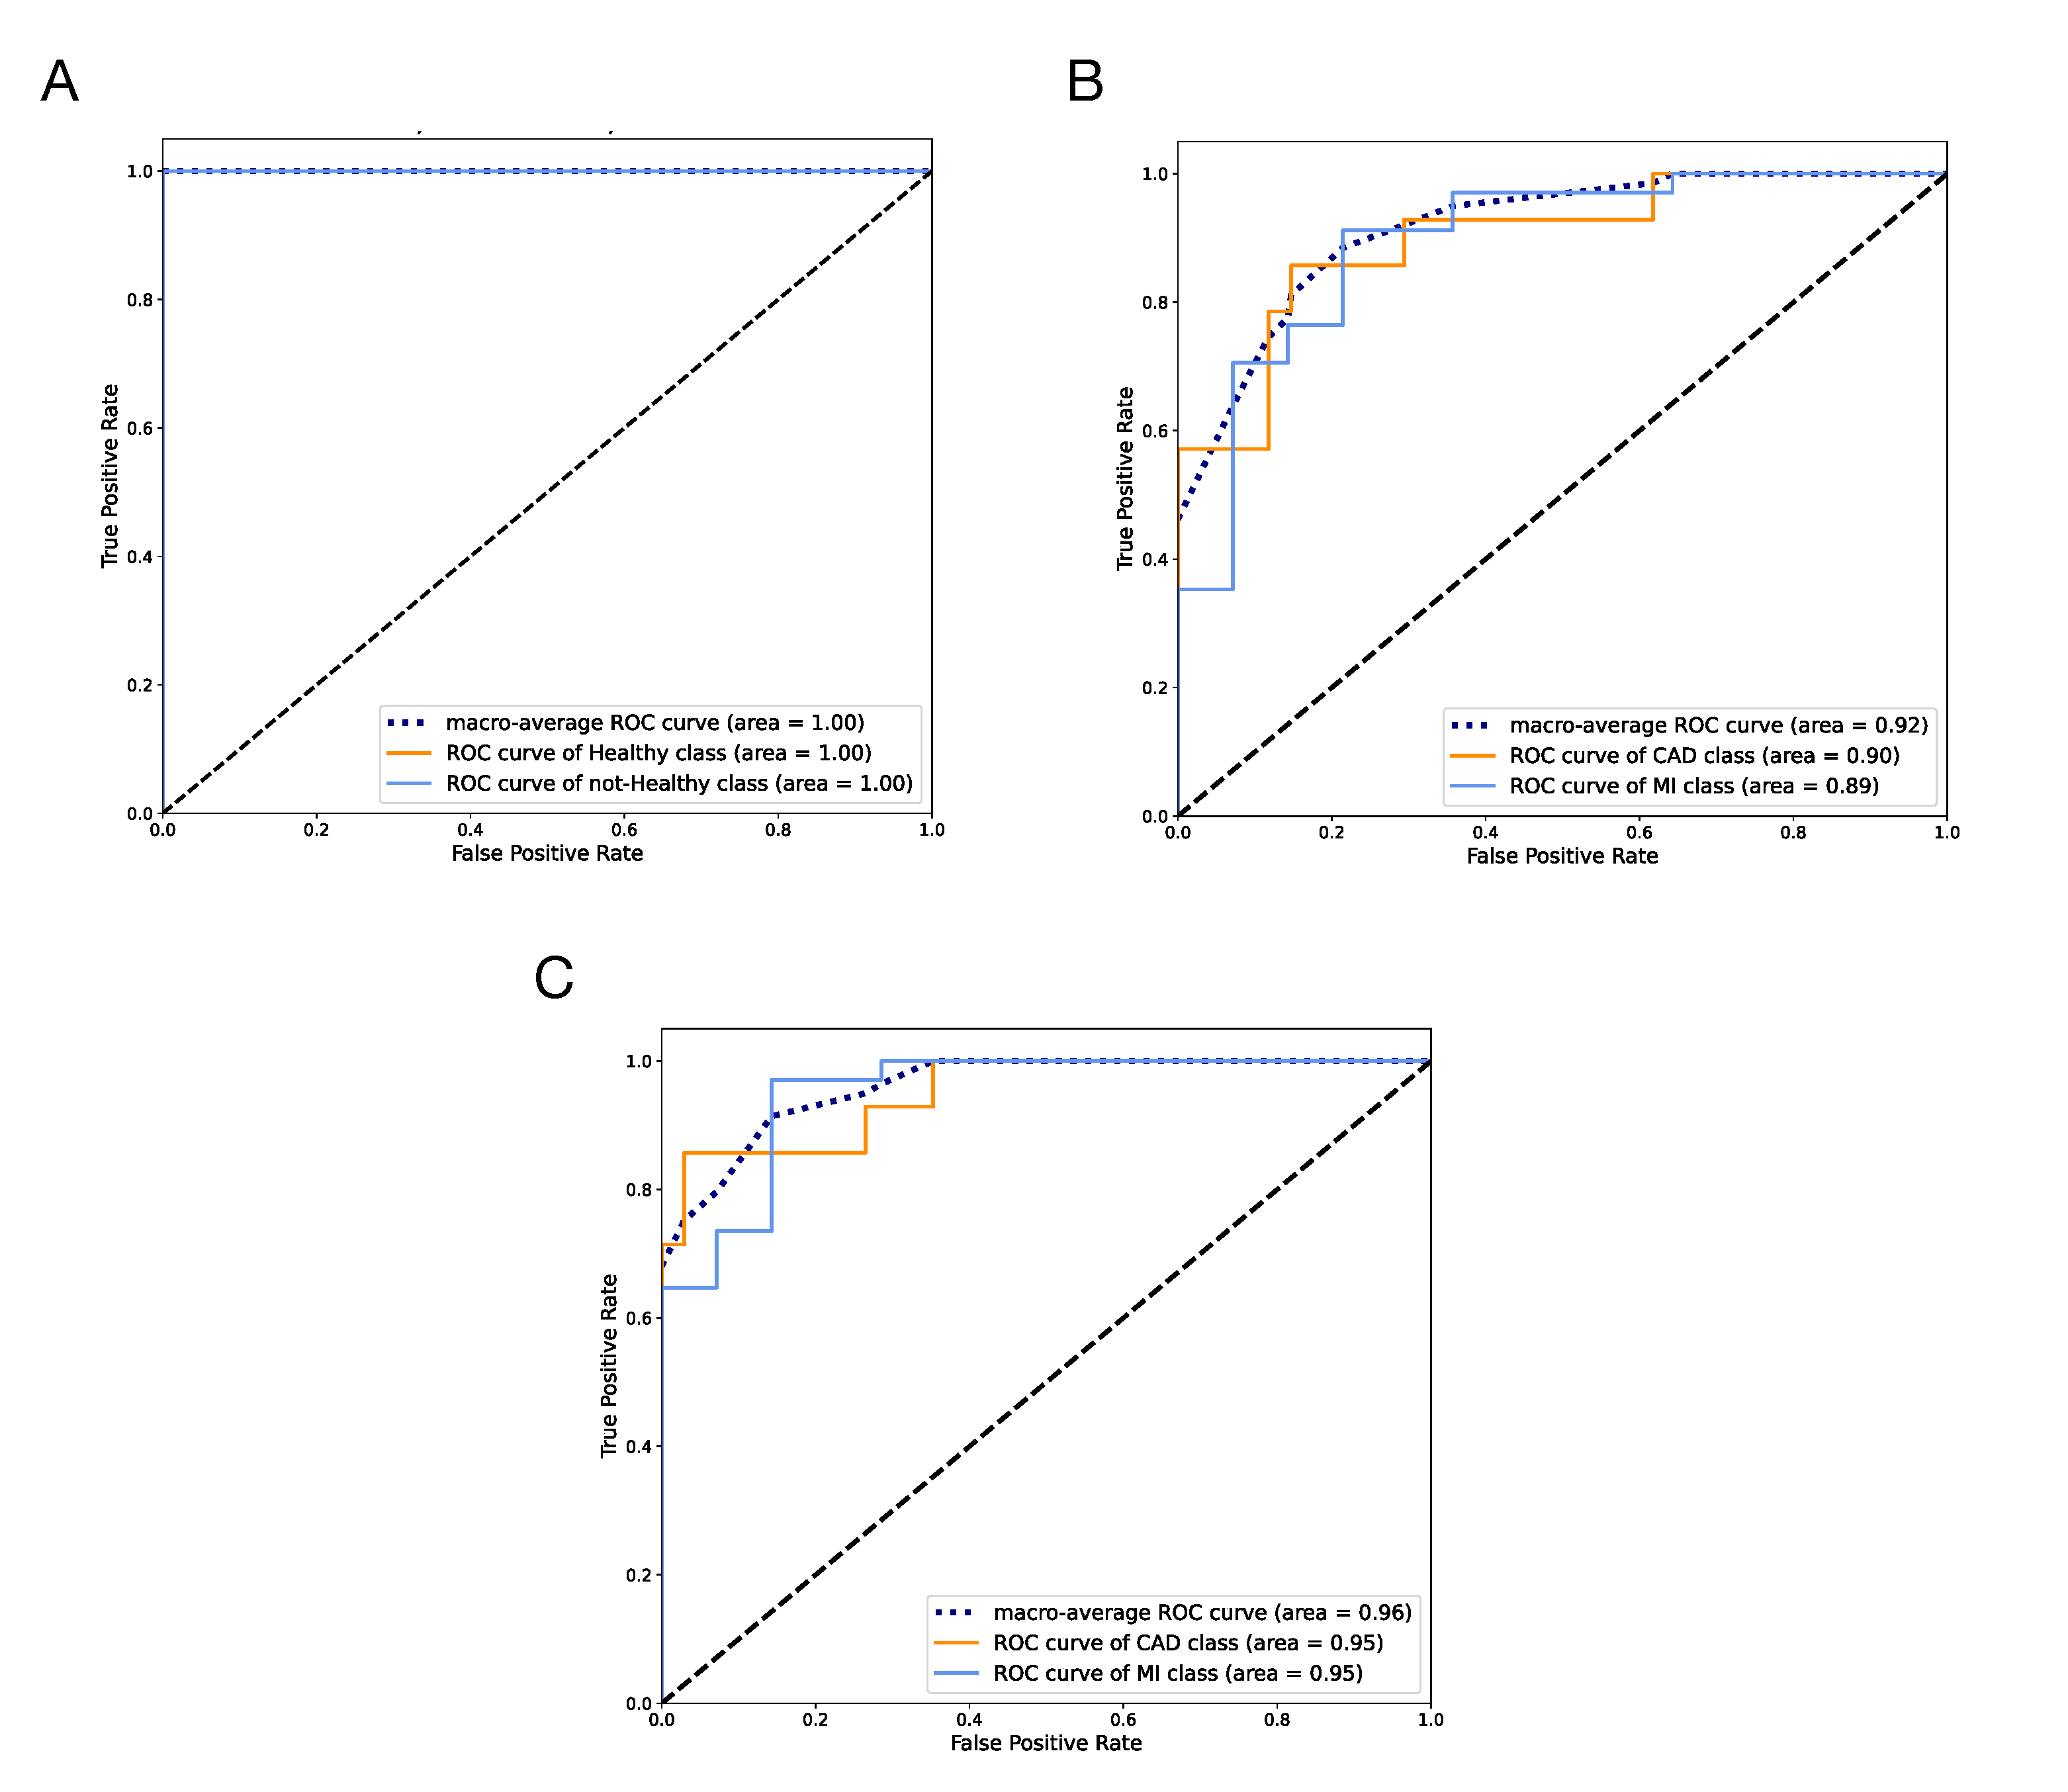
\includegraphics[width=0.95\linewidth]{../../ML/Pics/AUC best model ROCs} 

}

\caption{ROC curve for the set of miRNAs selected by AUC on test set classification. (A) SVM with RBF kernel for healthy and not-healthy samples classification. (B) Logistic regression model for CAD and MI samples classification. (C) SVM with polynomial kernel for CAD and MI samples classification. }\label{fig:AUCROC}
\end{figure}

\begin{figure}

{\centering 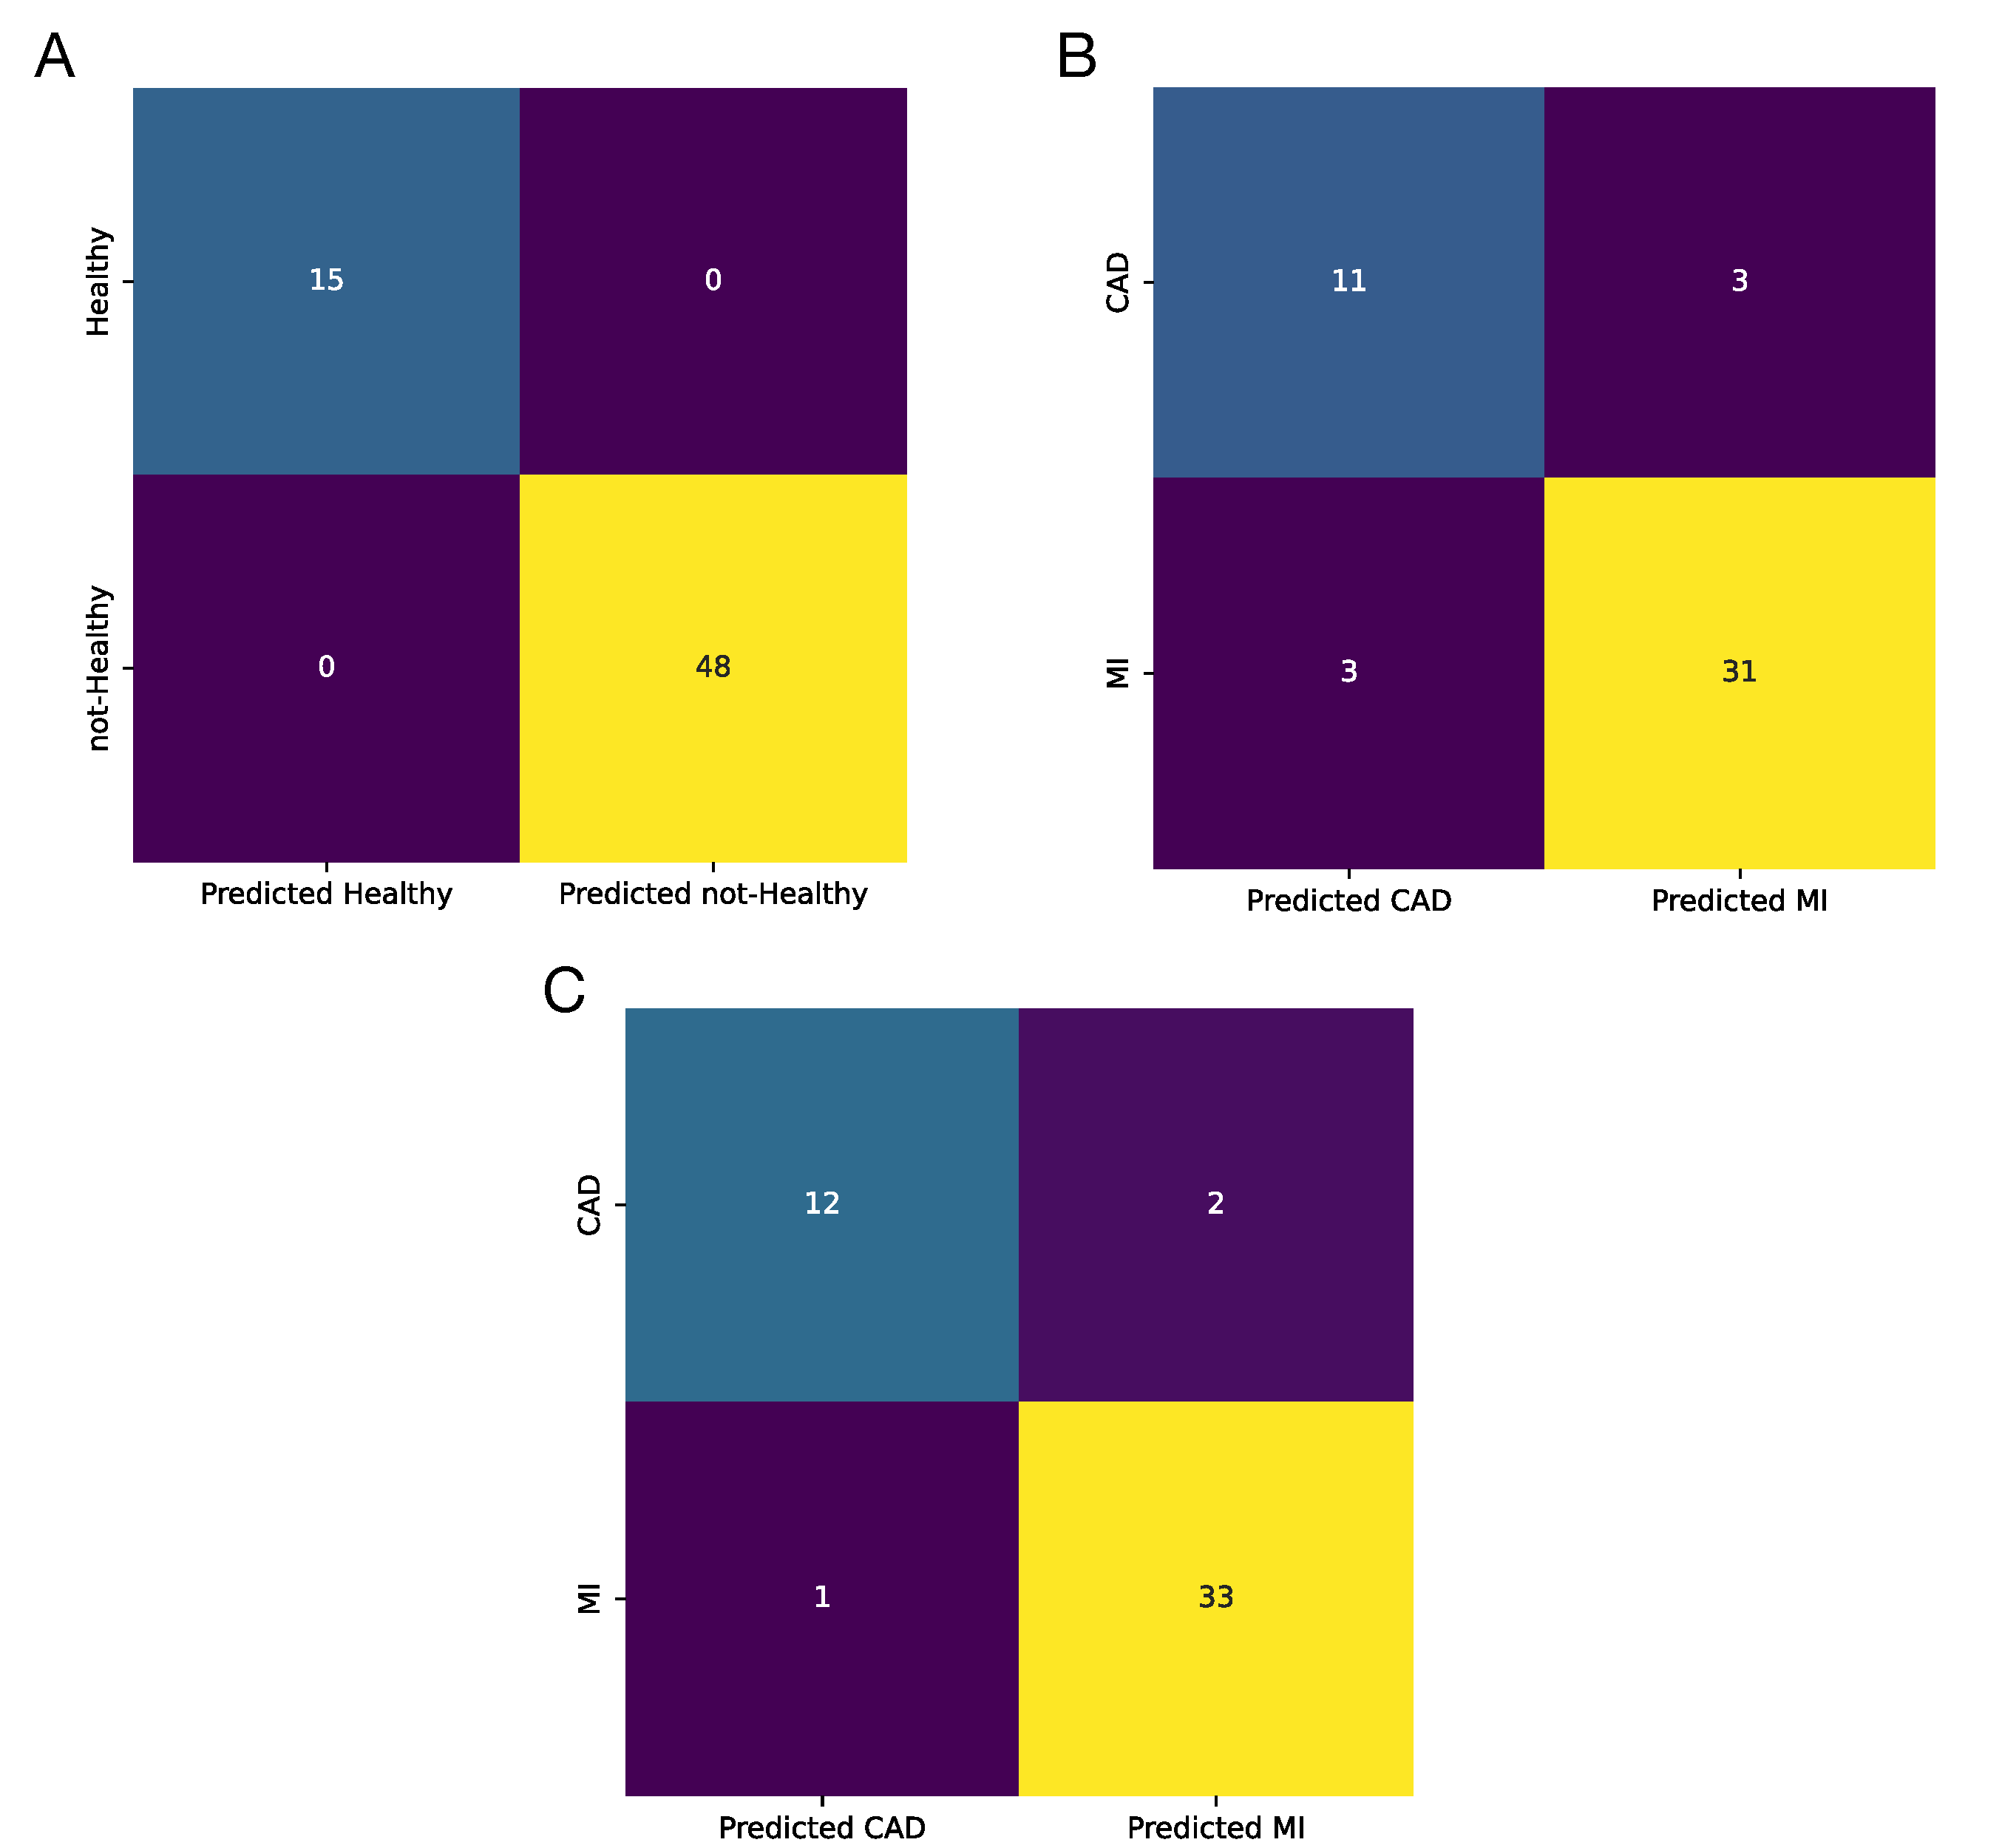
\includegraphics[width=0.9\linewidth]{../../ML/Pics/AUC Conf. matrix} 

}

\caption{Confusion matrix on the test set for (A) SVM with RBF kernel for healthy and not-healthy samples classification. (B) Logistic regression model for CAD and MI samples classification. (C) SVM with polynomial kernel for CAD and MI samples classification.}\label{fig:AUCCF}
\end{figure}

\hypertarget{second-layer-for-isolation-of-mi-samples-from-cad-samples}{%
\paragraph{Second layer for isolation of MI samples from CAD
samples}\label{second-layer-for-isolation-of-mi-samples-from-cad-samples}}

To find the best model for training the best set, different models were
trained using their pre-set values. Their AUC and accuracy results on
the test set are presented in Figure @ref(fig:AUCmodels). The best model
from the AUC point-of-view was the LR and from the accuracy
point-of-view, it was the SVM model with a polynomial kernel. For the LR
model the AUC and accuracy were 0.92 and 0.81, respectively; and for the
SVM model with a polynomial kernel, the values were 0.91 and 0.84,
respectively. Both models were hyper-tuned and the ROC curve for their
best performance is presented in Figure @ref(fig:AUCROC)B and C. The AUC
and accuracy for the LR model increased to 0.94 and 0.88, respectively.
For the SVM model with a polynomial kernel, these values increased to
0.95 and 0.88, respectively (Table @ref(tab:AUCML)). The sensitivity for
the LR and SVM models were 1 and 0.97, respectively; and the specificity
for them was 0.57 and 0.64, respectively. The confusion matrix for both
models is illustrated in Figure @ref(fig:AUCCF)B and C.

\begin{figure}

{\centering \includegraphics[width=0.65\linewidth]{../../ML/Pics/Models AUC mirs} 

}

\caption{Area under the curve (AUC) and accuracy of different models trained with three miRNAs in DEGs on the test set.}\label{fig:AUCmodels}
\end{figure}

\begin{table}

\caption{\label{tab:AUCML}AUC-ROC and accuracy for SVM with the linear kernel as the best model trained with miRNAs selected based on their individual AUC-ROC on the train and test set before and after hyper-tuning}
\centering
\begin{tabu} to \linewidth {>{\centering}X>{\centering}X>{\centering}X>{\centering}X>{\centering}X>{\centering}X}
\toprule
\multicolumn{2}{c}{ } & \multicolumn{2}{c}{Pre-set parameters} & \multicolumn{2}{c}{Hyper-tuned} \\
\cmidrule(l{3pt}r{3pt}){3-4} \cmidrule(l{3pt}r{3pt}){5-6}
Model & Metrics & Train & Test & Train & Test\\
\midrule
LR & AUC-ROC & 0.90 & 0.92 & 0.91 & 0.94\\
 & Accuracy & 0.84 & 0.81 & 0.84 & 0.88\\
SVM & AUC-ROC & 0.90 & 0.91 & 0.91 & 0.95\\
(Polynomial Kernel) & Accuracy & 0.86 & 0.84 & 0.86 & 0.88\\
\bottomrule
\end{tabu}
\end{table}

\hypertarget{discussion}{%
\section{Discussion}\label{discussion}}

The prevalence of acute MI (AMI) can lead to high-rate mortality in the
clinical setting. However, early diagnosis and application of suitable
treatment protocols can reduce mortality and improve AMI prognosis
({``Cardiovascular Diseases ({CVDs})''} n.d.; Thygesen et al. 2018; Tsao
et al. 2022). Studies have suggested that changes in miRNA expression
may play a significant role in the progression of MI and the subsequent
remodeling (Laggerbauer and Engelhardt 2022). It is believed that the
expression of miRNAs is altered during the various biological processes
correlated with MI within the myocardium or other related tissues (Khan,
Gupta, and Mahapatra 2022). Although several research has been
concentrated on examining free circulating miRNAs in the serum samples
for the detection of cardiac tissue injuries (Kaur et al. 2020), more
information is needed to fully comprehend the miRNAs found in different
blood sub-components like plasma, platelets, and PBMCs. Based on
previous data, PBMCs are critically involved in plaque destabilization
and rupture as well as early inflammatory responses during MI (Mosallaei
et al. 2022; Hapke et al. 2022). Moreover, PBMCs have specific miRNA
profile that is altered under certain pathological conditions which are
great candidates as disease biomarkers (Mosallaei et al. 2022).

PBMCs can respond to several insulting conditions such as MI in the
least possible time with prominent changes in their miRNA profile
(Mosallaei et al. 2022). Considering the regulatory roles, subtle
changes in the transcription of miRNAs can be monitored even before
alteration in the levels of mRNAs and proteins (Schulte et al. 2020).
These features make the miRNAs an early-stage valid diagnostic tool for
the detection of minor and major cell injuries. To date, few studies
have been performed to compare the miRNA profiles in PBMCs belonging to
acute MI patients and other CADs and healthy samples to find a robust
set of identical miRNAs to differentiate these pathological conditions.

In this study, we combined three GEO datasets of healthy, CAD, and MI
samples. Having these samples set alongside bioinformatics analysis and
ML means, it is possible to identify potential biomarker sets and also
effective therapeutic targets. The results of the DEG analysis (Table
@ref(tab:DEGstab) and Figure @ref(fig:venn)) are proof of the close
relationship between the MI and CAD samples. Interestingly, functional
enrichment analysis demonstrated that DEGs in both healthy/CAD and
healthy/MI were strongly correlated to immune cell response which is a
major cellular part of PBMCs. Here, two different sets of miRNAs were
used as biomarker sets for sample classification. miR-21; miR-32; and
miR-186 were selected as differentially expressed miRNAs, and miR-21;
miR-29a; miR-142; miR155; miR-197; and miR-320c1 were selected according
to their AUC values. As shown in Figure @ref(fig:miRROC), all other
miRNAs selected with both approaches had AUC-ROC over 0.9 for the
isolation of healthy and not-healthy samples except for miR-142 and
miR-29a. Data confirmed that the real challenge is to classify CAD and
MI samples because of close overlap. Of 8 miRNAs under investigation in
both approaches except for miR-32, all miRNAs had an AUC-ROC over 0.8
for the discrimination of CAD and MI samples. Besides, the high AUC-ROC
values of miRNAs confirms their high potential as biomarkers.

ML models when trained with miRNA sets selected by both DEG and AUC
approaches showed better performance in the classification than each
miRNA. To avoid unwanted complexity and poor predictive values, a
two-layer architecture was also designed. The first layer was for for
the discrimination of healthy from not-healthy samples, and the second
layer separated the CAD from MI candidates. As expected in both
approaches, a hyper-tuned SVM model could flawlessly separates healthy
from not-healthy samples using distinct miRNAs sets. The ML models were
also capable of effectively separating CAD from MI patients. Although
both miRNA sets had nearly the same AUC-ROC with their best model, the
accuracy, sensitivity, and specificity were different. The model trained
with DEGs had better specificity, but the one trained with AUC-selected
miRNAs had slightly better accuracy and higher sensitivity. This
difference comes from the different strategies the selection of
biomarkers sets.

Numerous studies have reported different biological processes can affect
the expression of miRNAs in PBMCs. However, there are still
controversies regarding the exact role of miRNAs in the function of
immune cells and the correlation of specific pathological conditions
with miRNA profiles. Several studies have proved the activation of
specific miRNA types in PBMCs under cardiovascular events (S. Li et al.
2015; Yao et al. 2016; Liu et al. 2017; Horita, Farquharson, and Stephen
2021; Cai et al. 2020; Zhao et al. 2018; Bhansali et al. 2022). For
instance, there is evidence that the elevation of miR-186 suppresses the
expression of Cystathionine-\(\gamma\)-lyase, leading to the subsequent
secretion of pro-inflammatory cytokines and cellular lipid accumulation.
Besides, macrophage-derived miR-186 may promote atherosclerotic plaques
(Yao et al. 2016). In line with this claim, we found that miR-186 is
up-regulated in both CAD and MI candidates related to control
counterparts. Surprisingly, the obtained data indicated that the
expression of miR-186 is higher in CAD patients in comparison to MI
(Figure @ref(fig:DEMexp)), To be specific, miR-186 is the only
differentially expressed miRNA between CAD and MI, indicating its main
role in the promotion of atherosclerosis.

As mentioned before, miR-21 was also up-regulated in both MI and CAD
patients in comparison to healthy controls. Moreover, the expression
value of miR-21 was significantly higher in MI than that of the CAD
group (Table @ref(tab:mirExptable)). It is thought that the
up-regulation of miRNA-21 in PBMCs is a compensatory reaction to reduce
T\(_{reg}\) lymphocyte number in response to the reduction of
TGF\(\beta1\) secretion into the plasma through a
TGF\(\beta1\)/smad-independent pathway. In line with previous and
present data, miR-21 can modulate the activity of PBMCs following the
occurrence of cardiovascular diseases (S. Li et al. 2015).

Recent data have supported the elevation of miR-32 in CAD patients with
the calcification of coronary artery. Of note, miR-32 stimulates the
calcification of mouse vascular smooth muscle through the regulation of
bone morphogenetic protein-1, runt-related transcription factor-2
(RUNX2), osteopontin, and bone-specific phosphoprotein matrix GLA
protein (Liu et al. 2017). Likewise, there are some reports associated
with the activity of PBMC miR-32 under several pathologies (Zeng et al.
2021; Wang et al. 2020). The exact role of PBMC miR-32 after
cardiovascular events remained to be elucidated.

Molecular analyses have indicated the regulatory role of miRNAs selected
by the AUC approach in PBMCs after a cardiovascular event. As the only
common miRNA of the two sets, molecular function of miR-21 in CVDs was
covered in DEGs miRNA set. Based on numerous reports mir-29a can be
activated in different diseases (Horita, Farquharson, and Stephen
2021).Data analysis indicated that miR-29a is significantly up-regulated
in CAD patients in comparison to healthy and MI groups (Table
@ref(tab:mirExptable)). Increased miR-29a is associated with the
progression of atherosclerosis, and the combination of miR-29a and
ox-LDL was offered as a valid biomarker set for paraclinical
classification (Huang et al. 2016). However, the role of miR-29a in the
function of PBMCs in CAD patients has not been completely examined.

According to the present data (Table @ref(tab:mirExptable)), the
difference in miR-142 expression between MI/Healthy and CAD/Healthy was
not significant, but these values reached statistically significant in
MI as compared to CAD. Based on different reports, miR-142 is commonly
active in PBMCs. This miRNA directly targets and inhibits the expression
of Adenomatous Polyposis Coli, a negative WNT signaling pathway
regulator, contributing to the activation of the WNT signaling pathway
and cardiac fibroblast activation after myocardial ischemia (Cai et al.
2020).

We also noted that miR-155 is the only down-regulated miRNA among all
miRNAs in both CAD/healthy and MI/Healthy comparisons (Table
@ref(tab:mirExptable)). There are numerous reports on the
down-regulation of miR-155 in PBMCs after MI or in CAD patients.
Previous data suggested an inverse relationship between miR-155 levels
and the severity of the coronary artery condition (Zhang et al. 2015;
Zhao et al. 2018). Along with current data and previous findings, it is
postulated that miR-155 has a protective effect under pathological
conditions. This genetic element can control inflammation and thus
reduce tissue damage through its negative feedback effects on
inflammatory factors. These features coincide with the reduction of
atherosclerosis (Zhang et al. 2015).

Data indicated that miR-197 is also significantly up-regulated in both
CAD/healthy and MI/healthy groups. In previous studies, it has been
shown that miRNA-197 may play a critical role in regulating the
anti-inflammatory response of IL-35 by affecting pro/ anti-inflammatory
cytokine secretion, M1/M2 macrophage ratio, T\(_{reg}\) lymphocyte
proliferation, and T cell suppression suggesting the potential
diagnostic role of miR-197 in adverse cardiovascular events (Bhansali et
al. 2022). There are some reports about miR-320 role in the
physiopathology of cardiac fibrosis. Mechanistically, Molecular analyses
revealed that miR-320 might induce various effects by targeting PLEKHM3
and IFITM1 in cardiomyocytes and cardiac fibroblasts, respectively (F.
Li et al. 2021). However, there are no reports on miR-320c1 activity in
the cardiovascular system or PBMCs.

\hypertarget{conclusion}{%
\section{Conclusion}\label{conclusion}}

In summary, we derived a set of miRNA biomarkers by comparing MI samples
to both healthy and CAD samples. We found that the SVM model performed
best in both the first layer, which separated healthy and not-healthy
samples, and the second layer, which classified MI/CAD samples. The set
of miRNAs selected based on their AUC values had slightly better
performance in the second layer. Overall, our two-layer structure
achieved a weighted accuracy of 0.91. This demonstrates the potential
for combining bioinformatics and machine learning techniques to identify
novel biomarkers and gain a deeper understanding of myocardial
infarction.

\hypertarget{references}{%
\section{References}\label{references}}

\begin{align}
a^2+b^2=c^2
\end{align}

\hypertarget{refs}{}
\begin{CSLReferences}{1}{0}
\leavevmode\vadjust pre{\hypertarget{ref-197}{}}%
Bhansali, Shipra, Amit Kumar Yadav, Chetan Bakshi, and Veena Dhawan.
2022. {``Interleukin-35 {Mitigates} Ox-{LDL}-{Induced} {Proatherogenic}
{Effects} via {Modulating} {miRNAs} {Associated} with {Coronary}
{Artery} {Disease} ({CAD}).''} \emph{Cardiovascular Drugs and Therapy},
April. \url{https://doi.org/10.1007/s10557-022-07335-x}.

\leavevmode\vadjust pre{\hypertarget{ref-142}{}}%
Cai, Lidong, Gong Chao, Weifeng Li, Jumo Zhu, Fangfang Li, Baozhen Qi,
Yong Wei, et al. 2020. {``Activated {Cd4}+ {T} Cells-Derived Exosomal
{miR}-142-3p Boosts Post-Ischemic Ventricular Remodeling by Activating
Myofibroblast.''} \emph{Aging} 12 (8): 7380--96.
\url{https://doi.org/10.18632/aging.103084}.

\leavevmode\vadjust pre{\hypertarget{ref-75}{}}%
Canali, Raffaella, Lucia Natarelli, Guido Leoni, Elena Azzini, Raffaella
Comitato, Oezgur Sancak, Luca Barella, and Fabio Virgili. 2014.
{``Vitamin {C} Supplementation Modulates Gene Expression in Peripheral
Blood Mononuclear Cells Specifically Upon an Inflammatory Stimulus: A
Pilot Study in Healthy Subjects.''} \emph{Genes \& Nutrition} 9 (3):
390. \url{https://doi.org/10.1007/s12263-014-0390-x}.

\leavevmode\vadjust pre{\hypertarget{ref-CVD}{}}%
{``Cardiovascular Diseases ({CVDs}).''} n.d. Accessed March 12, 2023.
\url{https://www.who.int/news-room/fact-sheets/detail/cardiovascular-diseases-(cvds)}.

\leavevmode\vadjust pre{\hypertarget{ref-PBMC-miR}{}}%
Gao, Jie, Jia Liu, Ying Zhang, BaoYi Guan, Hua Qu, Hua Chai, WenTing
Wang, XiaoJuan Ma, and DaZhuo Shi. 2020. {``{PBMCs}-{Derived} {microRNA}
{Signature} as a {Prethrombotic} {Status} {Discriminator} in {Stable}
{Coronary} {Artery} {Disease}.''} \emph{Thrombosis and Haemostasis} 120
(01): 121--31. \url{https://doi.org/10.1055/s-0039-1700518}.

\leavevmode\vadjust pre{\hypertarget{ref-Meder23}{}}%
Hapke, Nils, Margarete Heinrichs, DiyaaElDin Ashour, Elena Vogel, Ulrich
Hofmann, Stefan Frantz, and Gustavo Campos Ramos. 2022.
{``Identification of a Novel Cardiac Epitope Triggering {T}-Cell
Responses in Patients with Myocardial Infarction.''} \emph{Journal of
Molecular and Cellular Cardiology} 173 (December): 25--29.
\url{https://doi.org/10.1016/j.yjmcc.2022.09.001}.

\leavevmode\vadjust pre{\hypertarget{ref-numpy}{}}%
Harris, Charles R., K. Jarrod Millman, Stéfan J. van der Walt, Ralf
Gommers, Pauli Virtanen, David Cournapeau, Eric Wieser, et al. 2020.
{``Array Programming with {NumPy}.''} \emph{Nature} 585 (7825): 357--62.
\url{https://doi.org/10.1038/s41586-020-2649-2}.

\leavevmode\vadjust pre{\hypertarget{ref-scikitopt}{}}%
Head, Tim, Manoj Kumar, Holger Nahrstaedt, Gilles Louppe, and Iaroslav
Shcherbatyi. 2021. \emph{Scikit-Optimize/Scikit-Optimize} (version
v0.9.0). Zenodo. \url{https://doi.org/10.5281/zenodo.5565057}.

\leavevmode\vadjust pre{\hypertarget{ref-29aa}{}}%
Horita, Masahiro, Colin Farquharson, and Louise A Stephen. 2021. {``The
Role of {miR}‐29 Family in Disease.''} \emph{Journal of Cellular
Biochemistry} 122 (7): 696--715.
\url{https://doi.org/10.1002/jcb.29896}.

\leavevmode\vadjust pre{\hypertarget{ref-29a}{}}%
Huang, Yu-Qing, An-Ping Cai, Ji-Yan Chen, Cheng Huang, Jie Li, and
Ying-Qing Feng. 2016. {``The {Relationship} of {Plasma} {miR}-29a and
{Oxidized} {Low} {Density} {Lipoprotein} with {Atherosclerosis}.''}
\emph{Cellular Physiology and Biochemistry} 40 (6): 1521--28.
\url{https://doi.org/10.1159/000453202}.

\leavevmode\vadjust pre{\hypertarget{ref-m2}{}}%
Kalayinia, Samira, Fateme Arjmand, Majid Maleki, Mahshid Malakootian,
and Chandra Pal Singh. 2021. {``{MicroRNAs}: Roles in Cardiovascular
Development and Disease.''} \emph{Cardiovascular Pathology} 50
(January): 107296. \url{https://doi.org/10.1016/j.carpath.2020.107296}.

\leavevmode\vadjust pre{\hypertarget{ref-11-15}{}}%
Kaur, Amanpreet, Sharon T Mackin, Kenny Schlosser, Fui Lin Wong, Malik
Elharram, Christian Delles, Duncan J Stewart, Natalie Dayan, Tara
Landry, and Louise Pilote. 2020. {``Systematic Review of {microRNA}
Biomarkers in Acute Coronary Syndrome and Stable Coronary Artery
Disease.''} \emph{Cardiovascular Research} 116 (6): 1113--24.
\url{https://doi.org/10.1093/cvr/cvz302}.

\leavevmode\vadjust pre{\hypertarget{ref-24}{}}%
Khan, Abrar A., Vinayak Gupta, and Nitish R. Mahapatra. 2022. {``Key
Regulatory {miRNAs} in Lipid Homeostasis: {Implications} for
Cardiometabolic Diseases and Development of Novel Therapeutics.''}
\emph{Drug Discovery Today} 27 (8): 2170--80.
\url{https://doi.org/10.1016/j.drudis.2022.05.003}.

\leavevmode\vadjust pre{\hypertarget{ref-23}{}}%
Laggerbauer, Bernhard, and Stefan Engelhardt. 2022. {``{MicroRNAs} as
Therapeutic Targets in Cardiovascular Disease.''} \emph{Journal of
Clinical Investigation} 132 (11): e159179.
\url{https://doi.org/10.1172/JCI159179}.

\leavevmode\vadjust pre{\hypertarget{ref-BER}{}}%
Lazar, C., S. Meganck, J. Taminau, D. Steenhoff, A. Coletta, C. Molter,
D. Y. Weiss-Solis, R. Duque, H. Bersini, and A. Nowe. 2013. {``Batch
Effect Removal Methods for Microarray Gene Expression Data Integration:
A Survey.''} \emph{Briefings in Bioinformatics} 14 (4): 469--90.
\url{https://doi.org/10.1093/bib/bbs037}.

\leavevmode\vadjust pre{\hypertarget{ref-320}{}}%
Li, Fang, Shan-Shan Li, Hui Chen, Jian-Zhi Zhao, Jie Hao, Jin-Ming Liu,
Xiu-Guang Zu, and Wei Cui. 2021. {``{miR}-320 Accelerates Chronic Heart
Failure with Cardiac Fibrosis Through Activation of the {Il6}/{Stat3}
Axis.''} \emph{Aging} 13 (18): 22516--27.
\url{https://doi.org/10.18632/aging.203562}.

\leavevmode\vadjust pre{\hypertarget{ref-21}{}}%
Li, Sihui, Qian Fan, Shaolin He, Tingting Tang, Yuhua Liao, and
Jiangjiao Xie. 2015. {``{MicroRNA}-21 {Negatively} {Regulates} {Treg}
{Cells} {Through} a {TGF}-\(\beta1\)/{Smad}-{Independent} {Pathway} in
{Patients} with {Coronary} {Heart} {Disease}.''} \emph{Cellular
Physiology and Biochemistry} 37 (3): 866--78.
\url{https://doi.org/10.1159/000430214}.

\leavevmode\vadjust pre{\hypertarget{ref-32-2}{}}%
Liu, Jianghua, Xinhua Xiao, Yingying Shen, Ling Chen, Canxin Xu, Heng
Zhao, Ying Wu, et al. 2017. {``{MicroRNA}-32 Promotes Calcification in
Vascular Smooth Muscle Cells: {Implications} as a Novel Marker for
Coronary Artery Calcification.''} Edited by Yin Tintut. \emph{PLOS ONE}
12 (3): e0174138. \url{https://doi.org/10.1371/journal.pone.0174138}.

\leavevmode\vadjust pre{\hypertarget{ref-67}{}}%
Maciejak, Agata, Marek Kiliszek, Marcin Michalak, Dorota Tulacz,
Grzegorz Opolski, Krzysztof Matlak, Slawomir Dobrzycki, Agnieszka
Segiet, Monika Gora, and Beata Burzynska. 2015. {``Gene Expression
Profiling Reveals Potential Prognostic Biomarkers Associated with the
Progression of Heart Failure.''} \emph{Genome Medicine} 7 (1): 26.
\url{https://doi.org/10.1186/s13073-015-0149-z}.

\leavevmode\vadjust pre{\hypertarget{ref-09}{}}%
Matone, Alice, Colm M. O'Grada, Eugene T. Dillon, Ciara Morris, Miriam
F. Ryan, Marianne Walsh, Eileen R. Gibney, et al. 2015. {``Body Mass
Index Mediates Inflammatory Response to Acute Dietary Challenges.''}
\emph{Molecular Nutrition \& Food Research} 59 (11): 2279--92.
\url{https://doi.org/10.1002/mnfr.201500184}.

\leavevmode\vadjust pre{\hypertarget{ref-fRMA}{}}%
McCall, M. N., B. M. Bolstad, and R. A. Irizarry. 2010. {``Frozen Robust
Multiarray Analysis ({fRMA}).''} \emph{Biostatistics} 11 (2): 242--53.
\url{https://doi.org/10.1093/biostatistics/kxp059}.

\leavevmode\vadjust pre{\hypertarget{ref-Barcode}{}}%
McCall, Matthew N., Karan Uppal, Harris A. Jaffee, Michael J. Zilliox,
and Rafael A. Irizarry. 2011. {``The {Gene} {Expression} {Barcode}:
Leveraging Public Data Repositories to Begin Cataloging the Human and
Murine Transcriptomes.''} \emph{Nucleic Acids Research} 39 (suppl\_1):
D1011--15. \url{https://doi.org/10.1093/nar/gkq1259}.

\leavevmode\vadjust pre{\hypertarget{ref-pandas}{}}%
McKinney, Wes. 2010. {``{D}ata {S}tructures for {S}tatistical
{C}omputing in {P}ython.''} In \emph{{P}roceedings of the 9th {P}ython
in {S}cience {C}onference}, edited by Stéfan van der Walt and Jarrod
Millman, 56--61.
\href{https://doi.org/\%2010.25080/Majora-92bf1922-00a\%20}{https://doi.org/
10.25080/Majora-92bf1922-00a }.

\leavevmode\vadjust pre{\hypertarget{ref-Meder6}{}}%
Mosallaei, Meysam, Naeim Ehtesham, Shima Rahimirad, Mostafa Saghi, Nasim
Vatandoost, and Sharifeh Khosravi. 2022. {``{PBMCs}: A New Source of
Diagnostic and Prognostic Biomarkers.''} \emph{Archives of Physiology
and Biochemistry} 128 (4): 1081--87.
\url{https://doi.org/10.1080/13813455.2020.1752257}.

\leavevmode\vadjust pre{\hypertarget{ref-scikit-learn}{}}%
Pedregosa, F., G. Varoquaux, A. Gramfort, V. Michel, B. Thirion, O.
Grisel, M. Blondel, et al. 2011. {``Scikit-Learn: Machine Learning in
{P}ython.''} \emph{Journal of Machine Learning Research} 12: 2825--30.

\leavevmode\vadjust pre{\hypertarget{ref-ML}{}}%
Reel, Parminder S., Smarti Reel, Ewan Pearson, Emanuele Trucco, and
Emily Jefferson. 2021. {``Using Machine Learning Approaches for
Multi-Omics Data Analysis: {A} Review.''} \emph{Biotechnology Advances}
49 (July): 107739.
\url{https://doi.org/10.1016/j.biotechadv.2021.107739}.

\leavevmode\vadjust pre{\hypertarget{ref-miR}{}}%
Schulte, Christian, Temo Barwari, Abhishek Joshi, Tanja Zeller, and
Manuel Mayr. 2020. {``Noncoding {RNAs} Versus {Protein} {Biomarkers} in
{Cardiovascular} {Disease}.''} \emph{Trends in Molecular Medicine} 26
(6): 583--96. \url{https://doi.org/10.1016/j.molmed.2020.02.001}.

\leavevmode\vadjust pre{\hypertarget{ref-m1}{}}%
Schulte, Christian, Mahir Karakas, and Tanja Zeller. 2017.
{``{microRNAs} in Cardiovascular Disease -- Clinical Application.''}
\emph{Clinical Chemistry and Laboratory Medicine (CCLM)} 55 (5).
\url{https://doi.org/10.1515/cclm-2016-0576}.

\leavevmode\vadjust pre{\hypertarget{ref-36}{}}%
Soler-Botija, Carolina, Carolina Gálvez-Montón, and Antoni Bayés-Genís.
2019. {``Epigenetic {Biomarkers} in {Cardiovascular} {Diseases}.''}
\emph{Frontiers in Genetics} 10 (October): 950.
\url{https://doi.org/10.3389/fgene.2019.00950}.

\leavevmode\vadjust pre{\hypertarget{ref-17}{}}%
Thygesen, Kristian, Joseph S. Alpert, Allan S. Jaffe, Bernard R.
Chaitman, Jeroen J. Bax, David A. Morrow, Harvey D. White, and The
Executive Group on behalf of the Joint European Society of Cardiology
(ESC)/American College of Cardiology (ACC)/American Heart Association
(AHA)/World Heart Federation (WHF) Task Force for the Universal
Definition of Myocardial Infarction. 2018. {``Fourth {Universal}
{Definition} of {Myocardial} {Infarction} (2018).''} \emph{Circulation}
138 (20). \url{https://doi.org/10.1161/CIR.0000000000000617}.

\leavevmode\vadjust pre{\hypertarget{ref-ML-Bio}{}}%
Torun, Furkan M., Sebastian Virreira Winter, Sophia Doll, Felix M.
Riese, Artem Vorobyev, Johannes B. Mueller-Reif, Philipp E. Geyer, and
Maximilian T. Strauss. 2023. {``Transparent {Exploration} of {Machine}
{Learning} for {Biomarker} {Discovery} from {Proteomics} and {Omics}
{Data}.''} \emph{Journal of Proteome Research} 22 (2): 359--67.
\url{https://doi.org/10.1021/acs.jproteome.2c00473}.

\leavevmode\vadjust pre{\hypertarget{ref-18}{}}%
Tsao, Connie W., Aaron W. Aday, Zaid I. Almarzooq, Alvaro Alonso, Andrea
Z. Beaton, Marcio S. Bittencourt, Amelia K. Boehme, et al. 2022.
{``Heart {Disease} and {Stroke} {Statistics}---2022 {Update}: {A}
{Report} {From} the {American} {Heart} {Association}.''}
\emph{Circulation} 145 (8).
\url{https://doi.org/10.1161/CIR.0000000000001052}.

\leavevmode\vadjust pre{\hypertarget{ref-32}{}}%
Wang, Dan, Ting Zeng, Zhi Lin, Lu Yan, Fenglin Wang, Lanlan Tang, Leyuan
Wang, Daolin Tang, Pan Chen, and Minghua Yang. 2020. {``Long Non-Coding
{RNA} {Snhg5} Regulates Chemotherapy Resistance Through the
{miR}-32/{Dnajb9} Axis in Acute Myeloid Leukemia.''} \emph{Biomedicine
\& Pharmacotherapy} 123 (March): 109802.
\url{https://doi.org/10.1016/j.biopha.2019.109802}.

\leavevmode\vadjust pre{\hypertarget{ref-186}{}}%
Yao, Yan, Xin Zhang, Hai-peng Chen, Liang Li, Wei Xie, Gang Lan,
Zhen-wang Zhao, Xi-Long Zheng, Zong-bao Wang, and Chao-ke Tang. 2016.
{``{MicroRNA}-186 Promotes Macrophage Lipid Accumulation and Secretion
of Pro-Inflammatory Cytokines by Targeting Cystathionine
\(\gamma\)-Lyase in {THP}-1 Macrophages.''} \emph{Atherosclerosis} 250
(July): 122--32.
\url{https://doi.org/10.1016/j.atherosclerosis.2016.04.030}.

\leavevmode\vadjust pre{\hypertarget{ref-Macro}{}}%
Yap, Jonathan, Jason Irei, Javier Lozano-Gerona, Selena Vanapruks,
Tianmai Bishop, and William A. Boisvert. 2023. {``Macrophages in Cardiac
Remodelling After Myocardial Infarction.''} \emph{Nature Reviews
Cardiology}, January. \url{https://doi.org/10.1038/s41569-022-00823-5}.

\leavevmode\vadjust pre{\hypertarget{ref-magic}{}}%
Zeng, Zl, Qingyun Zhu, Zhibo Zhao, Xuyu Zu, and Jianghua Liu. 2021.
{``Magic and Mystery of {microRNA}‐32.''} \emph{Journal of Cellular and
Molecular Medicine} 25 (18): 8588--8601.
\url{https://doi.org/10.1111/jcmm.16861}.

\leavevmode\vadjust pre{\hypertarget{ref-155-2}{}}%
Zhang, Yu-Hui, Liang-Hua Xia, Jia-Mei Jin, Ming Zong, Ming Chen, and Bo
Zhang. 2015. {``Expression Level of {miR}--155 in Peripheral Blood.''}
\emph{Asian Pacific Journal of Tropical Medicine} 8 (3): 214--19.
\url{https://doi.org/10.1016/S1995-7645(14)60318-7}.

\leavevmode\vadjust pre{\hypertarget{ref-155-3}{}}%
Zhao, Duo, Jing Zhao, Jiangbin Sun, Yanling Su, Jinfeng Jian, Huaan Ye,
Jiawang Lin, Zongda Yang, Jiatao Feng, and Zhiping Wang. 2018. {``The
Expression Level of {miR}-155 in Plasma and Peripheral Blood Mononuclear
Cells in Coronary Artery Disease Patients and the Associations of These
Levels with the Apoptosis Rate of Peripheral Blood Mononuclear Cells.''}
\emph{Experimental and Therapeutic Medicine}, September.
\url{https://doi.org/10.3892/etm.2018.6797}.

\end{CSLReferences}


\bibliographystyle{spmpsci}
\bibliography{ForArticleRefrence.bib,discussion.bib,Introduction.bib}


\end{document}
